\documentclass[journal]{IEEEtran}
\usepackage{amsmath,amssymb,amsfonts}
\usepackage{array}
\usepackage{booktabs}
\usepackage{multirow}
\usepackage{cite}
\usepackage{url}
\usepackage{graphicx}
\usepackage[caption=false,font=normalsize,labelfont=sf,textfont=sf]{subfig}
\usepackage{tikz}
\usetikzlibrary{arrows.meta, positioning, shapes, fit, calc}
\usepackage{balance}
\usepackage{mathtools}
\usepackage{algorithm}
\usepackage{algpseudocode}
\usepackage[hypertexnames=false]{hyperref}

\newtheorem{definition}{Definition}
\newtheorem{principle}{Principle}

\DeclareMathOperator{\ECE}{ECE}

\begin{document}

\title{FAIR-BETH: A Fair Thresholding and Ablation Protocol for Behavioral Malicious-Process Detection under Distribution Shift}

\author{\emph{St\'{e}phane Ga\"{e}l R.} Ekodeck, \emph{Vivien Beyala} Kamgang, \emph{Serge Alain} Eb\'{e}l\'{e}, \emph{Ulrich Joel} Atchiengang Ngueyep,  \emph{St\'{e}phane Willy} Mossebo Tcheunteu,  \emph{Damaris Belle} M. Fotso,  \emph{Arthur Ulrich} Ewane and \emph{Julius Marcellin} Nkenlifack,~\IEEEmembership{Member,~IEEE,}
\thanks{The opinions expressed here are entirely those of the authors. This research received no external funding. The authors declare no conflicts of interest. \emph{(\textbf{Corresponding author:} St\'{e}phane Ga\"{e}l R. Ekodeck)}. \\
Author Contributions: Conceptualization, methodology, software, validation, formal analysis, investigation, data curation, and writing---original draft preparation, \emph{S.G.R.E.} and \emph{U.J.A.N.}; conceptualization, methodology, and writing---review and editing, \emph{S.A.E.} and \emph{V.B.K.}; formal analysis and investigation, \emph{S.W.M.T.} and \emph{D.B.M.F.}; data curation and validation, \emph{A.U.E.}; supervision, project administration, and writing---review and editing, \emph{J.M.N.} All authors have read and approved the article.
\par \emph{St\'{e}phane Ga\"{e}l R.} Ekodeck is with Department of Computer Science, LIRIMA, TEAM GRIMCAPE, University of Yaound\'{e} I, Yaound\'{e}, Cameroon; IRD, UMI, UMMISCO, IRD France Nord, F-93143 Bondy, France; Sorbonne Universit\'{e}s, Univ. Paris 06, UMI 209, UMMISCO, F-75005 Paris, France. (ORCID: 0000-0002-8094-8832, e-mail: stephane-gael.ekodeck@facsciences-uy1.cm).
\par \emph{Vivien Beyala} Kamgang is with RTU-Mathematics and Computer Science, and Department of Computer Science-HTTC, The University of Bertoua, Bertoua, Cameroon; RUFCEA(UR-IFIA)-University of Dschang, Dschang, Cameroon. (ORCID: 0000-0002-3644-1866, e-mail: vivsxx@univ-bertoua.cm).
\par \emph{Serge Alain} Eb\'{e}l\'{e} is with Department of Computer Science, LIRIMA, TEAM GRIMCAPE, University of Yaound\'{e} I, Yaound\'{e}, Cameroon; IRD, UMI, UMMISCO, IRD France Nord, F-93143 Bondy, France; Sorbonne Universit\'{e}s, Univ. Paris 06, UMI 209, UMMISCO, F-75005 Paris, France. (ORCID: 0000-0001-7036-7068, e-mail: serge-alain.ebele@facsciences-uy1.cm).
\par \emph{Ulrich Joel} Atchiengang, \emph{St\'{e}phane Willy} Mossebo Tcheunteu, \emph{Damaris Belle} M. Fotso, and \emph{Arthur Ulrich} Ewane are with University of Yaound\'{e} I, LIRIMA, TEAM GRIMCAPE, Yaound\'{e}, Cameroon.
\par \emph{Julius Marcellin} Nkenlifack is with RUFCEA(UR-IFIA)-University of Dschang, Dschang, Cameroon; RTU-Mathematics and Computer Science, The University of Bertoua, Bertoua, Cameroon. (ORCID: 0000-0003-3322-4687, e-mail: marcellin.nkenlifack@gmail.com).}}

\markboth{IEEE Transactions on Information Forensics and Security,~Vol.~xx, No.~xx, 2026}%
{Ekodeck \MakeLowercase{\textit{et al.}}: FAIR-BETH for Behavioral Malicious-Process Detection}

\maketitle

\begin{abstract}
Ransomware-oriented endpoint defense often motivates behavioral detection because hashes and signatures are fragile, but behavioral pipelines are frequently evaluated under thresholding protocols that make the operational conclusion ambiguous. This paper introduces FAIR-BETH, an instance of a general FAIR-X evaluation contract for behavioral security datasets under distribution shift. FAIR-BETH combines label-field exclusion, development-only vocabulary fitting, explicit ATT\&CK claim boundaries, held-out score calibration, common threshold policies, baseline parity, bootstrap uncertainty, and diagnostic gaps that quantify whether fusion adds value over a strong tabular baseline. We compare an Isolation Forest, a GRU autoencoder, score-only fusion, tabular Random Forests, meta fusion, ExtraTrees, gradient-boosting variants, a multilayer perceptron, and XGBoost. The official BETH training and validation splits contain no malicious process after aggregation, while the official test split contains 121 malicious processes out of 198. We therefore use the supplementary 2021may files only to build an enriched development pool and keep the official test split isolated. Under a common validation-FPR threshold policy, RF-500 and TabRF obtain similar F1 point estimates (0.7241 and 0.7210), with overlapping bootstrap intervals; MetaRF is lower (F1 = 0.6756), so fusion does not provide evidence of improvement. Additional BETH audits add held-out feature attribution, prefix detection, cost-sensitive thresholding, calibration reliability, feature-space stress tests, and host/temporal split checks. To test whether the protocol generalizes beyond BETH, we also apply it to MalBehavD-V1, an independent Cuckoo-sandbox API-call dataset with 1\,285 benign and 1\,285 malware samples; the full-sequence Random Forest obtains AUC 0.9902, AP 0.9922, and F1 0.9512 at a validation-FPR threshold, with repeated-split median F1 0.9533. The contribution is therefore not a new ransomware-family classifier, but a reusable evaluation contract and diagnostic audit for making behavioral malicious-process results defensible.
\end{abstract}

\begin{IEEEkeywords}
Malicious-process detection, ransomware-oriented defense, behavioral analysis, BETH dataset, anomaly detection, calibration, threshold selection, distribution shift, Random Forest, GRU autoencoder.
\end{IEEEkeywords}

\section{Introduction}
\label{sec:intro}

Ransomware defense remains a difficult endpoint-security problem because modern ransomware families are not static artifacts. Operators and affiliates recompile payloads, change packers, adjust command-line launchers, and vary execution environments. Static signatures, hashes, and portable-executable features are fast and useful in a layered defense, but they are brittle when the payload is repacked, recompiled, or delivered through an intermediate loader \cite{sikorski2012,anderson2018}. Behavioral monitoring is therefore attractive: instead of trying to identify a file before execution, a detector observes process creation, file operations, network activity, registry access, return codes, and temporal patterns that occur while software runs.

The appeal of behavioral malicious-process detection is also its main evaluation difficulty. In a controlled benchmark, the detector is asked to separate malicious and benign behavior; in deployment, it must do so under distribution shift, severe class imbalance, missing labels, and business constraints on false positives. A method that ranks malicious processes above benign ones may still be unusable if its threshold is selected on a validation set with a different prevalence. Conversely, a method that appears weak at a default threshold can become useful when threshold selection is tied to a validation false-positive budget. The same numerical score can therefore support different scientific claims depending on how the operating point is chosen.

This paper studies that issue on the BETH dataset \cite{highnam2021}, a real cybersecurity dataset designed for anomaly detection and out-of-distribution analysis. BETH contains low-level endpoint events across multiple hosts. It is an appropriate stress test for behavioral detection because it exposes process-level traces rather than static malware binaries. It is also a challenging benchmark because the official training and validation files contain no malicious process after the aggregation used in this paper, while the official test split is dominated by malicious processes. This creates an unusually strong mismatch between development and test distributions.

This paper addresses the evaluation problem through FAIR-BETH: a fair thresholding and ablation protocol that makes data access, feature construction, calibration, threshold selection, baseline parity, and uncertainty reporting explicit. The protocol is designed for BETH-like behavioral endpoint datasets where official splits are distribution-shifted and where the thresholding rule can materially change the operational interpretation of a detector.

The contribution is methodological and deliberately conservative:
\begin{itemize}
    \item We formalize FAIR-BETH as an instance of FAIR-X, a reusable evaluation contract that fixes data access, feature construction, calibration, thresholding, ablation, and uncertainty-reporting rules before final test labels are evaluated.
    \item We define a process-level behavioral feature space that uses only observable fields available in both official and supplementary BETH files. The ground-truth columns \texttt{sus} and \texttt{evil} are never used as predictors.
    \item We use MITRE ATT\&CK as response context rather than as a supervised predictor, because BETH does not provide validated ATT\&CK technique labels or documented event-to-technique mapping rules.
    \item We evaluate all supervised models under the same threshold policies: validation-FPR budget and validation-max-F1. This prevents a meta-model from gaining an artificial advantage through more favorable threshold selection.
    \item We introduce three audit diagnostics: the tabular-dominance gap, the score-compression gap, and threshold sensitivity. These quantities convert the qualitative claim ``fusion helps'' into a testable numerical statement.
    \item We report ranking metrics, thresholded metrics, confusion matrices, and nonparametric 95\% bootstrap confidence intervals \cite{efron1994}.
    \item We add stronger tabular baselines, including ExtraTrees, gradient boosting, an MLP, and XGBoost. RF-500 and TabRF are essentially tied under the main threshold policy, while score-only fusion and neural reconstruction are materially weaker.
    \item We validate the protocol on MalBehavD-V1 \cite{maniriho2023,malbehavd2023}, an independent Windows API-call sequence dataset, including repeated splits, prefix-length evaluation, and permutation feature attribution.
    \item We add BETH-specific limit-lifting audits: TabRF attribution, prefix detection, cost-sensitive thresholding, feature-space stress tests, and host/temporal split robustness.
\end{itemize}

This positioning matters because a defensible security-ML result must make clear what the experiment proves, what it does not prove, and which conclusions survive fair baselines. FAIR-BETH turns that requirement into an executable protocol. On the BETH configuration studied here, robust process aggregation and threshold discipline matter more than architectural complexity.

\section{Background and Problem Setting}
\label{sec:background}

\subsection{Behavioral Ransomware Detection}

Behavioral detection monitors actions rather than static bytes. A ransomware process may create or modify many files, enumerate directories, spawn child processes, open network connections, or invoke scripting interpreters. These actions are not unique to malware: backup agents, compilers, indexers, installers, and administrative scripts can produce high-volume file and process activity. The detection problem is therefore not merely whether a suspicious event exists, but whether a process-level pattern is sufficiently different from benign behavior to justify an alert.

The common modeling approaches include unsupervised anomaly detection, supervised classification, and sequence modeling. Isolation Forest \cite{liu2008} recursively partitions feature space and gives higher anomaly scores to samples isolated with shorter paths. It is attractive when malicious labels are scarce but does not output calibrated probabilities. Autoencoders, including recurrent autoencoders, learn to reconstruct normal sequences and use reconstruction error as an anomaly score \cite{cho2014,du2017}. Supervised classifiers such as Random Forests \cite{breiman2001} can exploit labels when available but may overfit benchmark-specific artifacts unless the split design is carefully controlled.

\subsection{Calibration and Operating Thresholds}

Ranking metrics such as AUC-ROC and Average Precision (AP) summarize score orderings. They do not specify an operating point. In an endpoint system, a score must be converted to an action: alert, isolate, suspend, or ignore. This requires a threshold. Threshold selection is especially sensitive when validation and test prevalence differ. A default threshold of 0.5 is rarely meaningful for anomaly scores and may also be inappropriate for class-weighted classifiers.

Calibration maps raw scores into probability-like quantities. Platt scaling \cite{platt1999} fits a logistic regression on a calibration set; expected calibration error (ECE) bins predictions and compares confidence to empirical accuracy \cite{guo2017}. In extreme imbalance, however, calibration can become numerically fragile. If a calibration fold contains only a handful of positives, the fitted probabilities may cluster near the base rate, and binned calibration estimates can have high variance. We therefore treat calibration as score normalization, not as evidence that the resulting probabilities are reliable risk estimates.

\subsection{Evaluation under Distribution Shift}

The BETH dataset was designed for anomaly detection and out-of-distribution analysis \cite{highnam2021}. This is important. In many benchmark papers, train and test splits are implicitly treated as exchangeable. In BETH, the official train/validation/test structure does not behave like an ordinary IID split after process aggregation. The official training and validation files contain no malicious process in our process-level representation; the official test file contains a majority of malicious processes. This creates a difficult but useful setting: the model cannot rely on an ordinary validation set to tune a malicious operating point.

We therefore distinguish between three evaluation concepts:
\begin{definition}[Ranking evaluation]
A ranking evaluation measures how well a model orders test processes by maliciousness, independent of any threshold.
\end{definition}

\begin{definition}[Thresholded evaluation]
A thresholded evaluation measures binary decisions after the threshold has been fixed using development data.
\end{definition}

\begin{definition}[Defensible threshold policy]
A threshold policy is defensible when every model being compared receives the same access to validation data and the threshold is fixed before test labels are used.
\end{definition}

The third definition drives the rest of the paper. We report multiple threshold policies, but we do not compare a meta-classifier tuned on validation FPR against a baseline left at a default threshold.

\section{Related Work and Positioning}
\label{sec:related}

\subsection{Static Malware Learning and Its Limits}

Static malware learning uses hashes, byte n-grams, imported functions, strings, headers, entropy profiles, and portable-executable metadata. Datasets such as EMBER \cite{anderson2018} made static malware-learning research more reproducible by providing feature extraction and baseline models. Static features are attractive because they can be computed before execution and can scale to large file repositories. They are also operationally important because an endpoint product should stop known malware as early as possible.

Ransomware, however, exposes a limitation of purely static reasoning. A ransomware campaign can reuse behavior while changing packaging. A loader can alter the observed file without changing the downstream encryption logic. A static classifier may generalize across some transformations but cannot observe runtime intent directly. Behavioral detection is therefore not a replacement for static detection; it is a complementary layer that becomes important when the file-level signal is weak, hidden, or unavailable. BETH is aligned with this behavioral layer because it does not provide raw binaries or PE features.

\subsection{Unsupervised Anomaly Detection}

Unsupervised anomaly detection is compelling in security because positive labels are scarce and expensive. Isolation Forest is a common baseline because it is simple, fast, and robust to high-dimensional tabular inputs \cite{liu2008}. The general anomaly-detection literature warns, however, that an anomaly is not necessarily an attack \cite{chandola2009}. A rare benign administrative action can be highly anomalous; a repeated malicious behavior can be statistically ordinary inside the dataset used for training.

This distinction explains why an unsupervised detector can fail under BETH distribution shift. If the benign development pool contains diverse administrative processes and the malicious test processes are internally regular, an Isolation Forest may rank benign processes as more anomalous. Such a failure is not surprising; it is a known mismatch between anomaly and maliciousness. The value of reporting it is that it prevents the paper from claiming an unsupervised branch is useful merely because it is architecturally plausible.

\subsection{Sequence Models for Logs}

Sequence models for logs, such as recurrent networks and transformer-style models, are often motivated by the observation that event order matters. DeepLog \cite{du2017} showed that sequence prediction can be effective for log anomaly detection. A GRU autoencoder uses a similar intuition: if the model reconstructs normal event sequences well, high reconstruction error may indicate abnormal behavior. This is a reasonable hypothesis for endpoint traces because a process is not just a bag of events; the order of file, process, and network operations can encode execution semantics.

The present results show that this hypothesis is not sufficient on its own. The GRU-AE obtains AUC 0.3913 on the official test split. One explanation is that eventId sequences in BETH are low-cardinality and regular enough that benign and malicious processes share many local patterns. Another explanation is that process-level event histograms already capture most of the discriminative signal available under this aggregation. A third explanation is that the sequence model was trained only on benign processes from a development distribution that does not match the official test distribution. These explanations are not mutually exclusive.

\subsection{Random Forests in Security Datasets}

Random Forests \cite{breiman2001} remain strong baselines in many tabular security datasets. They handle nonlinear interactions, tolerate mixed feature scales, provide stable performance with limited tuning, and are less data-hungry than neural models. In the context of BETH, a Random Forest can exploit interactions between event histograms and process-level scalar statistics. For example, a high event rate may be benign for a short-lived system process but suspicious when paired with a particular distribution of file and process events.

Because Random Forests are so strong on tabular data, any hybrid pipeline must compare against them carefully. A weak baseline makes a complex model appear more useful than it is. A default threshold on a class-weighted Random Forest is also insufficient: the default class prediction may be conservative under extreme imbalance. FAIR-BETH therefore evaluates TabRF and stronger tabular alternatives under the same threshold policies as MetaRF.

\subsection{Gradient Boosting and Tabular Deep Baselines}

Modern tabular baselines include boosted trees such as XGBoost \cite{chen2016xgboost} and LightGBM \cite{ke2017lightgbm}, as well as neural tabular learners such as TabNet \cite{arik2021tabnet}. These methods are relevant because the BETH representation used here is primarily tabular after process aggregation. The additional audit therefore includes executable comparisons with XGBoost, ExtraTrees, scikit-learn gradient boosting, histogram gradient boosting, a multilayer perceptron, and a larger 500-tree Random Forest. LightGBM and TabNet are discussed as related tabular model families but are not required dependencies in the reproducibility package.

\subsection{Security-ML Evaluation Pitfalls}

FAIR-X is not intended to rediscover generic machine-learning hygiene. It is a concrete evaluation contract for a narrower failure mode in behavioral security benchmarks: a complex detector can appear useful because feature construction, threshold selection, baseline strength, or claim boundaries differ across models. This positioning follows the concerns raised by Arp et al. \cite{arp2022}, who document recurring pitfalls in machine-learning-based security evaluation. FAIR-X turns part of that guidance into executable checks for this setting: no test-label influence on feature construction or thresholds, identical threshold policies for compared models, explicit baseline parity, uncertainty intervals, diagnostic gaps, and claim-boundary audits. Its novelty is therefore not the individual rule ``do not leak test labels,'' but the way these rules are combined with threshold and fusion diagnostics for distribution-shifted behavioral process detection.

\subsection{Calibration in Security}

Calibration is often discussed as if it converts classifier scores into trustworthy probabilities. In high-stakes security, this interpretation should be used carefully. Platt scaling can improve score monotonicity and make scores comparable, but its reliability depends on the calibration data. When a calibration fold contains six positives, each positive contributes materially to the fitted logistic curve. ECE is also unstable because bins may contain very few positive examples. The present paper therefore uses calibration as a procedural normalization step and reports calibration fragility as a finding.

\subsection{MITRE ATT\&CK as Response Context}

MITRE ATT\&CK provides a useful language for tactics and techniques \cite{mitre2023,strom2018}. It helps analysts connect low-level telemetry to adversary behavior and response playbooks. Yet ATT\&CK technique labels are not automatically available in BETH. Mapping an event identifier such as \texttt{openat}, \texttt{execve}, or \texttt{connect} to a technique requires context. The same system call can be benign, suspicious, or malicious depending on arguments, parent process, user, host role, and temporal context.

For that reason, this paper uses ATT\&CK as an analyst-facing response vocabulary rather than as a supervised feature source. This separates two different questions: whether a detector can classify malicious processes, and whether an alert can be translated into ATT\&CK language through validated telemetry semantics or documented analyst rules. The former is evaluated; the latter is discussed as operational design.

\section{Formal Problem Definition}
\label{sec:formal}

Let $\mathcal{E}$ be the set of raw endpoint events. Each event $e$ has a timestamp, a host identifier, a process identifier, a parent-process identifier, an event identifier, a textual argument field, a return value, and a label annotation. A process group is:
\[
G_i = \{e \in \mathcal{E}: host(e)=h_i, processId(e)=p_i\}.
\]
The process-level label is:
\[
y_i = \max_{e\in G_i}\mathbf{1}\{evil(e)=1\}.
\]
The model receives a feature representation $x_i=f(G_i)$ and outputs a score $s_i=g(x_i)$, where higher scores are intended to indicate higher maliciousness.

The evaluation problem has two layers. The ranking layer measures whether:
\[
s_i > s_j \quad \text{for malicious } i \text{ and benign } j.
\]
The decision layer chooses a threshold $\tau$ and predicts:
\[
\hat{y}_i(\tau)=\mathbf{1}\{s_i \geq \tau\}.
\]
The threshold $\tau$ must be a function of development data only:
\[
\tau = T(\mathcal{D}_{\text{train}},\mathcal{D}_{\text{cal}},\mathcal{D}_{\text{val}}),
\]
and not a function of official test labels.

For the FPR-budget policy, let $\mathcal{V}_0$ be the benign subset of \texttt{val\_strat}. We choose:
\[
\tau_{\mathrm{FPR}}=\max\{\tau: \frac{1}{|\mathcal{V}_0|}\sum_{i\in \mathcal{V}_0}\mathbf{1}\{s_i\geq\tau\}\leq \alpha\},
\]
with $\alpha=0.05$. For the validation-F1 policy, let $\mathcal{V}$ be the complete stratified validation fold. We choose:
\[
\tau_{F1}=\arg\max_{\tau \in \mathcal{T}} F1(\mathcal{V},\tau),
\]
where $\mathcal{T}$ is the set of observed validation scores. The FPR policy encodes an operational constraint; the F1 policy encodes a data-driven trade-off that is less stable when positives are scarce.

This formalization clarifies the main fairness requirement. If two models are compared, the mapping $T$ from validation scores to threshold must be the same type of mapping. Otherwise, the comparison confounds the classifier with the threshold policy.

\section{FAIR-BETH Protocol}
\label{sec:fairbeth}

FAIR-BETH is the protocol used in this paper to make BETH process-level behavioral evaluation defensible under distribution shift. It is not a new feature extractor or classifier. It is an evaluation contract: it specifies what information a model may use, how thresholds are selected, how baselines are compared, and which diagnostic quantities must be reported before claiming that a hybrid detector improves over a simpler baseline.

\subsection{General FAIR-X Evaluation Contract}
\label{sec:fairx_contract}

FAIR-BETH is an instance of a more general evaluation contract, denoted FAIR-X, for behavioral security datasets whose development and test distributions may differ. Let $\mathcal{D}_{dev}$ be all data available before final testing, $\mathcal{D}_{test}$ be the isolated final test set, $\mathcal{F}$ be a feature-construction operator, $\mathcal{T}$ be a threshold-selection operator, and $\mathcal{M}=\{M_1,\ldots,M_k\}$ be the candidate models. A FAIR-X experiment is the tuple
\[
\mathcal{E}=(\mathcal{D}_{dev},\mathcal{D}_{test},\mathcal{F},\mathcal{M},\mathcal{T},\mathcal{A}),
\]
where $\mathcal{A}$ is a declared audit set. The tuple is valid only if the following invariants hold before test evaluation:
\[
\mathcal{F}\perp Y_{test}, \qquad \mathcal{T}\perp Y_{test}, \qquad
\forall M_i,M_j\in\mathcal{M}: \mathcal{T}_i=\mathcal{T}_j
\]
for every model comparison used to support a scientific claim. The first two invariants exclude test-label leakage through feature construction and threshold selection. The third invariant enforces threshold fairness: a hybrid model cannot be compared against a baseline that receives a weaker operating-point policy.

The audit set $\mathcal{A}$ must include at least one baseline-parity audit, one threshold-sensitivity audit, and one uncertainty audit. For deployment-oriented claims, $\mathcal{A}$ should also include prefix latency, cost sensitivity, and split robustness. FAIR-BETH instantiates this contract with BETH process aggregation, a family of direct tabular baselines, MetaRF as the hybrid candidate, validation-FPR and validation-F1 threshold policies, bootstrap intervals, diagnostic gaps, and the limit-lifting audits in Section~\ref{sec:limit_lifting}. Figure~\ref{fig:fairx_protocol} summarizes the resulting contract.

\begin{definition}[FAIR-X improvement claim]
A model $M_a$ has a defensible improvement claim over $M_b$ under policy $\pi$ only if both models use the same admissible training information, the same threshold policy $\pi$, no test labels in feature construction or threshold selection, and the reported uncertainty does not contradict the claimed effect direction.
\end{definition}

\begin{principle}[Fusion burden of proof]
Under a FAIR-X contract, a hybrid detector does not earn its added complexity unless its test-set utility exceeds the strongest admissible non-hybrid baseline under the same threshold policy and audit set.
\end{principle}

The principle is operational rather than asymptotic. It defines the burden of proof used in this paper: MetaRF is not rejected because fusion is impossible; it fails because, under the same threshold policy and data access, it does not improve over the strongest admissible tabular baseline on the evaluated BETH configuration.

\begin{figure*}[t]
\centering
\resizebox{\textwidth}{!}{%
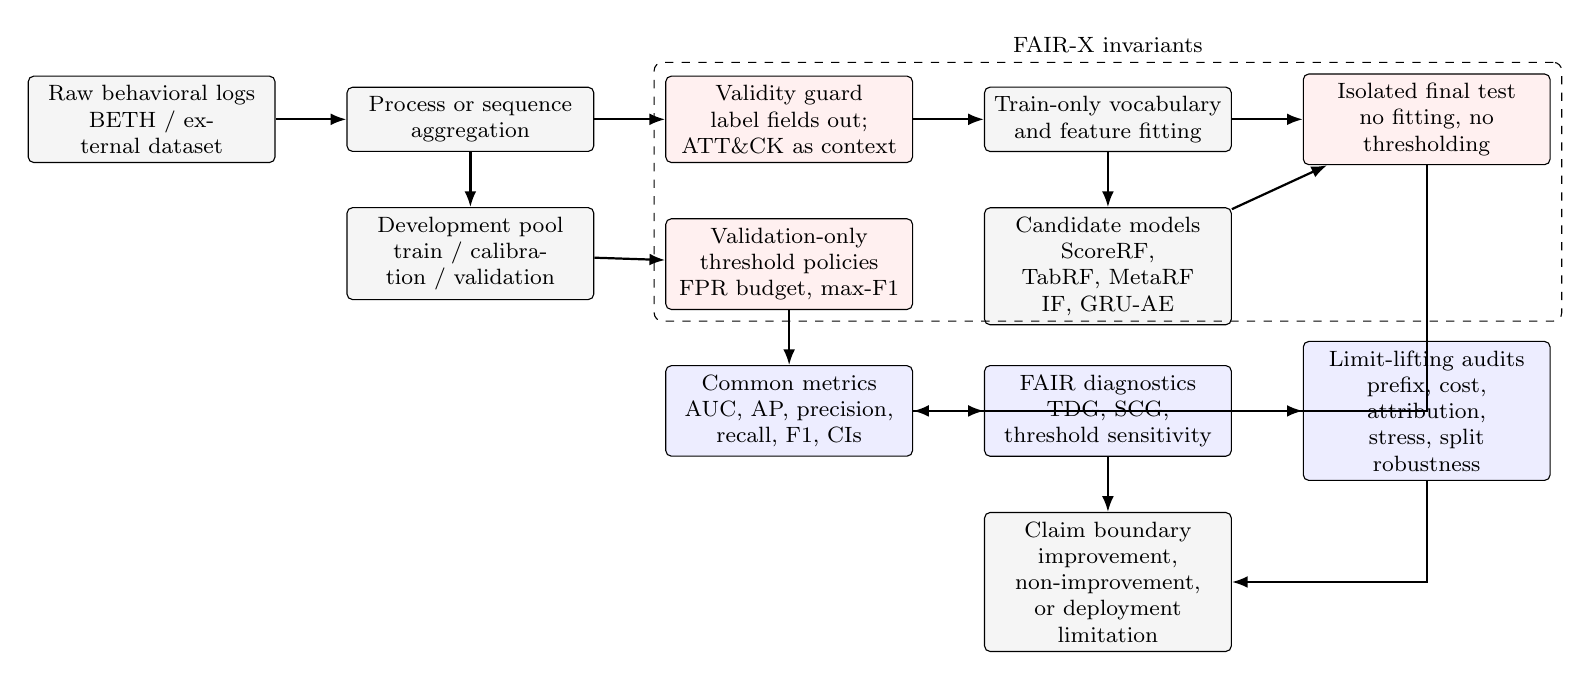
\begin{tikzpicture}[
    font=\footnotesize,
    node distance=7mm and 9mm,
    block/.style={draw, rounded corners=2pt, align=center, minimum height=8mm, text width=2.9cm, fill=gray!8},
    audit/.style={draw, rounded corners=2pt, align=center, minimum height=8mm, text width=2.9cm, fill=blue!7},
    lock/.style={draw, rounded corners=2pt, align=center, minimum height=8mm, text width=2.9cm, fill=red!6},
    arrow/.style={-{Latex[length=2mm]}, thick}
]
\node[block] (raw) {Raw behavioral logs\\BETH / external dataset};
\node[block, right=of raw] (aggregate) {Process or sequence\\aggregation};
\node[lock, right=of aggregate] (sanitize) {Validity guard\\label fields out;\\ATT\&CK as context};
\node[block, right=of sanitize] (features) {Train-only vocabulary\\and feature fitting};

\node[block, below=of aggregate] (dev) {Development pool\\train / calibration / validation};
\node[lock, below=of sanitize] (thresholds) {Validation-only\\threshold policies\\FPR budget, max-F1};
\node[block, below=of features] (models) {Candidate models\\ScoreRF, TabRF, MetaRF\\IF, GRU-AE};
\node[lock, right=of features] (test) {Isolated final test\\no fitting, no thresholding};

\node[audit, below=of thresholds] (metrics) {Common metrics\\AUC, AP, precision,\\recall, F1, CIs};
\node[audit, right=of metrics] (diagnostics) {FAIR diagnostics\\TDG, SCG,\\threshold sensitivity};
\node[audit, right=of diagnostics] (limits) {Limit-lifting audits\\prefix, cost, attribution,\\stress, split robustness};
\node[block, below=of diagnostics] (claims) {Claim boundary\\improvement, non-improvement,\\or deployment limitation};

\draw[arrow] (raw) -- (aggregate);
\draw[arrow] (aggregate) -- (sanitize);
\draw[arrow] (sanitize) -- (features);
\draw[arrow] (features) -- (test);
\draw[arrow] (aggregate) -- (dev);
\draw[arrow] (dev) -- (thresholds);
\draw[arrow] (features) -- (models);
\draw[arrow] (models) -- (test);
\draw[arrow] (thresholds) -- (metrics);
\draw[arrow] (test) |- (metrics);
\draw[arrow] (metrics) -- (diagnostics);
\draw[arrow] (diagnostics) -- (limits);
\draw[arrow] (diagnostics) -- (claims);
\draw[arrow] (limits) |- (claims);

\node[draw, dashed, rounded corners=3pt, fit=(sanitize)(thresholds)(test), inner sep=4pt, label={[font=\footnotesize]above:FAIR-X invariants}] {};
\end{tikzpicture}
}
\caption{FAIR-X/FAIR-BETH evaluation contract. Red blocks are non-negotiable validity guards; blue blocks are audits that determine whether a performance claim, negative result, or deployment boundary is defensible.}
\label{fig:fairx_protocol}
\end{figure*}

\subsection{Protocol Requirements}

The protocol has six requirements. First, the official test split is isolated from model fitting, calibration, threshold selection, feature-vocabulary construction, and model selection. Second, annotation columns such as \texttt{sus} and \texttt{evil} are used only to construct labels and never as predictors. Third, ATT\&CK-related annotations are used as predictive variables only when the dataset provides validated technique labels or documented mapping rules. Fourth, all models are evaluated under the same threshold policies. Fifth, every hybrid model is compared against the strongest reasonable non-hybrid baseline using the same data access and threshold policy. Sixth, uncertainty and failure modes are reported alongside point estimates. Algorithm~\ref{alg:fairbeth} gives the resulting execution order.

\begin{algorithm}[t]
\caption{FAIR-BETH evaluation protocol}
\label{alg:fairbeth}
\begin{algorithmic}[1]
\Require Official BETH train/validation/test files, supplementary development files, target FPR budget $\alpha$
\Ensure Test metrics, confidence intervals, and diagnostic gaps
\State Aggregate events by $(hostName, processId)$ and define process labels from \texttt{evil}
\State Keep annotation fields out of predictors and reserve ATT\&CK mappings for response context unless validated
\State Build an enriched development pool without using official test labels
\State Split development data into train, calibration, and stratified validation folds
\State Fit feature vocabularies and preprocessing transforms on development data only
\State Train raw detectors, supervised tabular baselines, score-only fusion, and meta-fusion
\State Calibrate raw detector scores on the calibration fold
\State Select $\tau_{\mathrm{FPR}}$ and $\tau_{F1}$ on the validation fold for every model
\State Evaluate all fixed models and thresholds once on the official test split
\State Compute ranking metrics, thresholded metrics, confusion matrices, bootstrap intervals, and diagnostic gaps
\end{algorithmic}
\end{algorithm}

\subsection{Diagnostic Gaps}

The novelty of FAIR-BETH is partly procedural and partly diagnostic. The diagnostic quantities below are designed to expose whether a complex detector actually adds information beyond a strong tabular baseline.

Let $M_{\mathrm{base}}$ denote the strongest admissible non-hybrid tabular baseline, $M_{\mathrm{score}}$ the score-only fusion model, $M_{\mathrm{meta}}$ the meta-fusion model, and $\pi$ a fixed threshold policy. The \emph{tabular-dominance gap} is:
\[
\mathrm{TDG}_{\pi}=F1(M_{\mathrm{base}},\pi)-F1(M_{\mathrm{meta}},\pi).
\]
A positive value means the hybrid meta-model does not improve over the tabular baseline under the same threshold policy. The \emph{score-compression gap} is:
\[
\mathrm{SCG}_{\pi}=F1(M_{\mathrm{base}},\pi)-F1(M_{\mathrm{score}},\pi).
\]
A large positive value means that detector scores compress away useful behavioral information. Finally, the \emph{threshold sensitivity} of model $M$ is:
\[
\mathrm{TS}_{M}=|F1(M,\tau_{\mathrm{FPR}})-F1(M,\tau_{F1})|.
\]
This measures how much the reported F1 changes when the validation objective changes. A large value warns that claims based on one threshold policy may not be stable.

These gaps deliberately use F1 because the main comparison concerns thresholded operational decisions. They do not replace AUC, AP, or confidence intervals. Rather, they summarize the practical question at the center of the experiment: after giving every model the same validation access, does fusion still help?

\subsection{Scope of the Protocol}

FAIR-BETH is intentionally narrow. It applies to process-level behavioral experiments on BETH-like endpoint logs where official splits are distribution-shifted and where threshold selection is part of the scientific claim. It does not by itself solve family attribution, direct cross-schema model transfer, malware-level evasion, or response safety. The additional audits quantify feature attribution, prefix latency, operational cost sensitivity, and split robustness, but those measurements remain evidence about the evaluated datasets rather than deployment certification. The purpose of FAIR-BETH is to prevent an avoidable methodological error: claiming novelty from a hybrid architecture when the measured gain comes from unequal thresholding, label leakage, or feature sources whose supervision or semantics are not available at deployment time.

\section{Dataset and Data Engineering}
\label{sec:data}

\subsection{BETH Files and Process-Level Labels}

BETH consists of low-level events with fields such as \texttt{timestamp}, \texttt{processId}, \texttt{parentProcessId}, \texttt{eventId}, \texttt{eventName}, \texttt{argsNum}, \texttt{returnValue}, \texttt{args}, \texttt{hostName}, \texttt{sus}, and \texttt{evil}. The official files and supplementary 2021may files do not have identical schemas: the official files include fields such as \texttt{threadId}, \texttt{mountNamespace}, and \texttt{stackAddresses}, while the supplementary files omit some of these fields. To avoid schema-dependent artifacts, we use only the fields present across the files needed for the experiment.

We aggregate events by the pair $(\texttt{hostName}, \texttt{processId})$. A process is labeled malicious if any event in the group has $\texttt{evil}=1$. The label fields are used only for this group label. They are excluded from all feature vectors. This choice is essential because \texttt{sus} and \texttt{evil} are annotations, not observables available to a deployed detector.

Table~\ref{tab:file_inventory} summarizes the event-level and process-level inventory used by the pipeline. The official training and validation files contain no malicious process after aggregation. The official test file contains 121 malicious processes out of 198. The supplementary 2021may files provide the positive development examples needed for calibration and validation, but they do not remove the distribution shift between development and official test.

\begin{table*}[t]
\centering
\caption{BETH file inventory after process aggregation. DNS files are excluded.}
\label{tab:file_inventory}
\begin{tabular}{lrrrrr}
\toprule
\textbf{File} & \textbf{Events} & \textbf{Evil events} & \textbf{Processes} & \textbf{Evil processes} & \textbf{Unique eventIds} \\
\midrule
labelled\_training\_data.csv & 763\,144 & 0 & 1\,179 & 0 & 32 \\
labelled\_validation\_data.csv & 188\,967 & 0 & 244 & 0 & 29 \\
labelled\_testing\_data.csv & 188\,967 & 158\,432 & 198 & 121 & 46 \\
labelled\_2021may-ubuntu.csv & 199\,222 & 0 & 298 & 0 & 17 \\
labelled\_2021may-ip-10-100-1-4.csv & 485\,241 & 4\,394 & 809 & 6 & 45 \\
labelled\_2021may-ip-10-100-1-26.csv & 378\,424 & 0 & 449 & 0 & 34 \\
labelled\_2021may-ip-10-100-1-95.csv & 479\,433 & 0 & 1\,124 & 0 & 38 \\
labelled\_2021may-ip-10-100-1-105.csv & 409\,931 & 5\,611 & 599 & 23 & 47 \\
labelled\_2021may-ip-10-100-1-186.csv & 713\,867 & 0 & 1\,505 & 0 & 33 \\
\bottomrule
\end{tabular}
\end{table*}

\subsection{Development and Test Protocol}

Because the official training and validation splits are monoclasse at process level, they cannot be used alone to train and calibrate supervised process-level detectors. We therefore construct an enriched development pool from the official training file plus the non-DNS supplementary 2021may files. The official test file remains isolated and is used only once for final evaluation.

The enriched development pool is split into:
\begin{itemize}
    \item \textbf{train} (65\%): model fitting and detector training;
    \item \textbf{cal} (20\%): Platt scaling and calibration diagnostics;
    \item \textbf{val\_strat} (15\%): threshold selection.
\end{itemize}
The split is stratified by process-level label. Table~\ref{tab:splits_new} gives the resulting process counts. The positive counts are small: 19 in train, 6 in calibration, and 4 in stratified validation. This is not ideal, but it is the only way to define a threshold without touching the official test labels. We explicitly report this as a limitation and use bootstrap intervals to avoid overclaiming precision.

\begin{table}[t]
\centering
\caption{Process-level splits used for model development and final evaluation.}
\label{tab:splits_new}
\begin{tabular}{lrrr}
\toprule
\textbf{Split} & \textbf{Total} & \textbf{Malicious} & \textbf{Rate} \\
\midrule
Train & 3\,782 & 19 & 0.50\% \\
Calibration & 1\,163 & 6 & 0.52\% \\
Stratified validation & 874 & 4 & 0.46\% \\
Official validation & 244 & 0 & 0.00\% \\
Official test & 198 & 121 & 61.11\% \\
\bottomrule
\end{tabular}
\end{table}

\subsection{Feature Construction}

For each process, we build a behavioral vector from scalar statistics and normalized event histograms. The final tabular vector has 61 dimensions: 13 scalar process statistics and 48 eventId histogram dimensions learned from the enriched development vocabulary. The scalar features are:
\begin{itemize}
    \item number of events;
    \item number of unique event identifiers;
    \item Shannon entropy of the event identifier distribution;
    \item mean, standard deviation, and maximum of \texttt{argsNum};
    \item mean and standard deviation of \texttt{returnValue};
    \item process duration;
    \item event rate;
    \item number of unique argument strings;
    \item mean argument-string length;
    \item number of unique parent process identifiers.
\end{itemize}

The histogram part of the feature vector is normalized by the number of events in the process. This prevents long processes from dominating solely because they contain more events. Process length remains available through $n_{\text{events}}$ and event rate.

\subsection{Sequence Representation}

For the GRU autoencoder, each process is represented as a sequence of event identifiers. Event identifiers are mapped to integer tokens. Token 0 is padding, and token 1 is reserved for unknown identifiers. The sequence length is set to the 95th percentile of training sequence lengths, which is 1\,152 events. Shorter sequences are padded. Longer sequences are uniformly sampled with evenly spaced indices. Uniform sampling avoids the strong bias introduced by truncating only the beginning or only the end of long traces.

\subsection{Why ATT\&CK Is Used as Response Context}

MITRE ATT\&CK is valuable for analyst interpretation and response planning \cite{mitre2023,strom2018}. However, BETH event identifiers do not include validated ATT\&CK technique labels or documented EDR mapping rules. Technique assignment depends on arguments, parent process, user, file path, network context, host role, and event sequence. The experiment therefore does not treat ATT\&CK technique IDs as supervised predictors. This is not a rejection of ATT\&CK; it is a boundary on what the present data can support. Section~\ref{sec:response} returns to ATT\&CK as a response taxonomy rather than as an evaluated predictive feature.

\section{Models}
\label{sec:models}

\subsection{Isolation Forest with Platt Scaling}

The first detector is an Isolation Forest \cite{liu2008} with 200 trees. The contamination parameter is set to the empirical malicious rate in the training fold. Input features are standardized using parameters learned on the training fold. The raw anomaly score is the negative of the scikit-learn \texttt{decision\_function}; larger values are intended to indicate greater abnormality. Because the score is not a probability, we fit Platt scaling on the calibration fold.

This detector is deliberately simple. It represents the hypothesis that malicious processes are isolated in process-level feature space without requiring many labels. If the detector fails, the failure is informative because it indicates that the malicious test processes are not merely outliers relative to the development processes.

\subsection{GRU Autoencoder with Platt Scaling}

The second detector is a GRU autoencoder trained only on benign training sequences. It has an embedding dimension of 32, hidden dimension of 64, one recurrent layer, and 42\,482 trainable parameters. The decoder reconstructs the input event sequence, and the anomaly score is the mean negative log-likelihood per non-padding token. We use Adam with learning rate $10^{-3}$, batch size 512, and early stopping against the official validation reconstruction loss. The official validation split contains only benign processes, so it is suitable for monitoring benign reconstruction but not for selecting a malicious operating threshold.

The autoencoder tests whether sequential order adds useful information beyond event histograms. A recurrent model should in principle capture local event ordering, repeated motifs, and unusual process trajectories. In practice, the results show that this sequence signal does not dominate the simpler tabular representation on BETH.

\subsection{Score-Only Random Forest}

The score-only Random Forest, denoted ScoreRF, uses only calibrated detector scores and their simple average as features. Its input is therefore:
\[
X_{\text{score}} = [p_{\text{IF}}, p_{\text{GRU}}, (p_{\text{IF}} + p_{\text{GRU}})/2].
\]
This model isolates the contribution of detector fusion. If ScoreRF performs well, score-level fusion is sufficient. If it performs poorly while direct tabular baselines perform well, the raw behavioral features contain information lost by the detector scores.

\subsection{Tabular Random Forest}

The tabular Random Forest, denoted TabRF, is a supervised classifier trained on the 61-dimensional process feature vector. It uses 200 trees, balanced class weights, no fixed maximum depth, and minimum leaf size 2. Inputs are standardized before fitting. Although Random Forests do not require feature scaling for split decisions, the same scaling interface is maintained across the codebase for reproducibility and comparability.

TabRF is the main ablation baseline, and RF-500 is added as a stronger tabular stress baseline. These are not weak baselines; they directly test whether the engineered process features are already sufficient. A hybrid model must beat the strongest admissible tabular baseline under the same threshold policy to justify added complexity.

\subsection{Meta Random Forest}

The meta Random Forest, denoted MetaRF, concatenates score-level features with the raw tabular vector:
\[
X_{\text{meta}} = [p_{\text{IF}}, p_{\text{GRU}}, p_{\text{avg}}, X_{\text{tab}}].
\]
It uses 300 trees, balanced class weights, and minimum leaf size 2. It is trained on the union of train and calibration folds after Platt scaling has been fit. The stratified validation fold is not used for fitting; it is reserved for threshold selection.

MetaRF is intentionally evaluated as an ablation, not as the presumed best model. The central question is whether adding calibrated detector scores to raw features improves over direct tabular learning. The answer in Section~\ref{sec:results} is no.

\section{Thresholding and Metrics}
\label{sec:thresholds}

\subsection{Threshold Policies}

We evaluate two threshold policies for every model:
\begin{itemize}
    \item \textbf{Validation-FPR budget}: choose the largest validation threshold satisfying $\mathrm{FPR} \leq 0.05$ on \texttt{val\_strat}.
    \item \textbf{Validation-max-F1}: choose the validation threshold that maximizes F1 on \texttt{val\_strat}.
\end{itemize}
Both policies are imperfect because \texttt{val\_strat} contains only four malicious processes. The FPR-budget policy is more operationally meaningful: it reflects the usual security requirement that false positives be limited before deployment. The max-F1 policy is reported as a sensitivity analysis and is not used as the main claim.

The critical methodological point is that both policies are applied to every model. This prevents the following common but invalid comparison: a meta-classifier is evaluated at a tuned threshold while the baseline is evaluated at 0.5. Such a comparison confounds model quality with threshold policy.

\subsection{Ranking and Thresholded Metrics}

We report AUC-ROC and AP as ranking metrics. AP is particularly relevant under class imbalance because it summarizes precision-recall behavior and is sensitive to the positive class prevalence \cite{saito2015}. For thresholded metrics we report precision, recall, F1, and the confusion matrix.

Let TP, FP, TN, and FN denote true positives, false positives, true negatives, and false negatives. The reported binary metrics are:
\[
\mathrm{Precision} = \frac{\mathrm{TP}}{\mathrm{TP}+\mathrm{FP}},
\quad
\mathrm{Recall} = \frac{\mathrm{TP}}{\mathrm{TP}+\mathrm{FN}},
\]
\[
F1 = \frac{2\cdot \mathrm{Precision}\cdot \mathrm{Recall}}{\mathrm{Precision}+\mathrm{Recall}}.
\]
When the denominator is zero, the metric is set to zero.

\subsection{Bootstrap Confidence Intervals}

The official test set contains only 198 processes. Point estimates can therefore be unstable. We compute nonparametric bootstrap confidence intervals by resampling the test processes with replacement 1\,000 times \cite{efron1994}. For each bootstrap sample containing both classes, we recompute AUC, AP, precision, recall, and F1 at the fixed threshold. The 2.5th and 97.5th percentiles define the 95\% interval.

The bootstrap is not a substitute for cross-dataset validation. It quantifies sampling uncertainty conditional on the test set. We use it to avoid overstating small differences such as AUC 0.736 versus 0.711. The separate MalBehavD-V1 experiment in Section~\ref{sec:external_malbehavd} tests whether the protocol itself transfers to a second behavioral schema; it is not used to claim direct BETH-model transfer.

\section{Implementation and Reproducibility}
\label{sec:implementation}

All experiments run on an HP ZBook 15 G5 with Intel Core i7-8750H CPU, 12 logical cores, 15.64 GB RAM, no GPU, Windows 11, Python 3.13.5, PyTorch 2.8.0+cpu, scikit-learn 1.7.2, pandas 2.3.1, NumPy 2.2.6, matplotlib 3.10.5, seaborn 0.13.2, tqdm 4.67.1, and psutil 7.0.0. The full CPU run, including preprocessing, GRU training, calibration, ablations, evaluation, and figure generation, completed in approximately 21 minutes on the test machine.

The code fixes the random seed at 42 for Python, NumPy, and PyTorch. The preprocessing stage writes five pickled datasets: train, calibration, stratified validation, official validation, and official test. The model stage writes detector outputs and fitted models. The evaluation stage writes a CSV table containing all metrics and confidence intervals, plus ROC, precision-recall, and confusion-matrix figures. This separation is useful because it prevents accidental reuse of test labels during model fitting and makes it possible to inspect each artifact independently.

\section{Results}
\label{sec:results}

\subsection{Full Quantitative Results}

Table~\ref{tab:full_results} gives the full test-set results for the original FAIR-BETH ablation set. Under the validation-FPR budget, TabRF obtains AUC 0.7360, AP 0.8270, precision 0.7500, recall 0.6942, and F1 0.7210. Its confusion matrix is TN=49, FP=28, FN=37, TP=84. MetaRF has lower AUC, AP, recall, and F1 under the same policy. ScoreRF improves over the unsupervised detectors but remains much weaker than TabRF.

\begin{table*}[t]
\centering
\caption{Complete test-set results with common threshold policies. Confidence intervals are 95\% nonparametric bootstrap intervals.}
\label{tab:full_results}
\begin{tabular}{llcccccc}
\toprule
\textbf{Model} & \textbf{Threshold policy} & \textbf{AUC} & \textbf{AP} & \textbf{Precision} & \textbf{Recall} & \textbf{F1} & \textbf{F1 95\% CI} \\
\midrule
IF-Platt & val-FPR budget & 0.3496 & 0.5195 & 0.3500 & 0.0579 & 0.0993 & [0.0303, 0.1727] \\
IF-Platt & val-max-F1 & 0.3496 & 0.5195 & 0.4590 & 0.2314 & 0.3077 & [0.2128, 0.3895] \\
GRUAE-Platt & val-FPR budget & 0.3913 & 0.5347 & 0.6250 & 0.0413 & 0.0775 & [0.0163, 0.1475] \\
GRUAE-Platt & val-max-F1 & 0.3913 & 0.5347 & 0.5638 & 0.4380 & 0.4930 & [0.4095, 0.5702] \\
SimpleAvg & val-FPR budget & 0.3402 & 0.5089 & 0.2778 & 0.0413 & 0.0719 & [0.0150, 0.1379] \\
SimpleAvg & val-max-F1 & 0.3402 & 0.5089 & 0.5060 & 0.3471 & 0.4118 & [0.3179, 0.5022] \\
ScoreRF & val-FPR budget & 0.5960 & 0.6846 & 0.6769 & 0.3636 & 0.4731 & [0.3825, 0.5650] \\
ScoreRF & val-max-F1 & 0.5960 & 0.6846 & 0.6852 & 0.3058 & 0.4229 & [0.3250, 0.5165] \\
\textbf{TabRF} & \textbf{val-FPR budget} & \textbf{0.7360} & \textbf{0.8270} & \textbf{0.7500} & \textbf{0.6942} & \textbf{0.7210} & \textbf{[0.6484, 0.7849]} \\
TabRF & val-max-F1 & 0.7360 & 0.8270 & 0.9583 & 0.3802 & 0.5444 & [0.4512, 0.6304] \\
MetaRF & val-FPR budget & 0.7113 & 0.8105 & 0.7308 & 0.6281 & 0.6756 & [0.5990, 0.7456] \\
MetaRF & val-max-F1 & 0.7113 & 0.8105 & 0.9474 & 0.2975 & 0.4528 & [0.3544, 0.5476] \\
\bottomrule
\end{tabular}
\end{table*}

The result contradicts the tempting narrative that a hybrid detector automatically improves over a tabular baseline. On this benchmark, with this split, and under common thresholding, detector-score fusion does not improve over direct tabular learning. This is the principal empirical finding.

\subsection{Comparison with Stronger Tabular Baselines}

Table~\ref{tab:sota_tabular} adds stronger tabular baselines trained on the same development information and evaluated under the same validation-FPR threshold policy. RF-500 obtains the highest F1 point estimate, 0.7241, but its interval overlaps TabRF's interval and the confusion matrices differ by only one benign decision. ExtraTrees has the best AUC and AP but selects a conservative operating point with lower recall. XGBoost, histogram gradient boosting, standard gradient boosting, and the MLP do not improve the thresholded F1 under this validation policy.

\begin{table*}[t]
\centering
\caption{Additional tabular baselines on the official BETH test split under the common validation-FPR threshold policy. Confidence intervals are 95\% nonparametric bootstrap intervals.}
\label{tab:sota_tabular}
\begin{tabular}{lcccccccc}
\toprule
\textbf{Model} & \textbf{AUC} & \textbf{AP} & \textbf{Precision} & \textbf{Recall} & \textbf{F1} & \textbf{F1 95\% CI} & \textbf{FP} & \textbf{FN} \\
\midrule
RF-500 & 0.7487 & 0.8342 & 0.7568 & 0.6942 & 0.7241 & [0.6572, 0.7835] & 27 & 37 \\
TabRF & 0.7360 & 0.8270 & 0.7500 & 0.6942 & 0.7210 & [0.6484, 0.7828] & 28 & 37 \\
MetaRF & 0.7113 & 0.8105 & 0.7308 & 0.6281 & 0.6756 & [0.5972, 0.7357] & 28 & 45 \\
ExtraTrees & 0.7973 & 0.8572 & 0.9649 & 0.4545 & 0.6180 & [0.5358, 0.6982] & 2 & 66 \\
HistGradientBoosting & 0.7106 & 0.8090 & 0.7033 & 0.5289 & 0.6038 & [0.5206, 0.6814] & 27 & 57 \\
XGBoost & 0.6717 & 0.7841 & 0.7176 & 0.5041 & 0.5922 & [0.5087, 0.6636] & 24 & 60 \\
MLP & 0.7865 & 0.8339 & 0.9231 & 0.3967 & 0.5549 & [0.4733, 0.6361] & 4 & 73 \\
GradientBoosting & 0.6153 & 0.7552 & 0.6571 & 0.3802 & 0.4817 & [0.3844, 0.5701] & 24 & 75 \\
ScoreRF & 0.5960 & 0.6846 & 0.6769 & 0.3636 & 0.4731 & [0.3771, 0.5651] & 21 & 77 \\
LogReg & 0.7698 & 0.8024 & 0.7059 & 0.0992 & 0.1739 & [0.0847, 0.2501] & 5 & 109 \\
\bottomrule
\end{tabular}
\end{table*}

These comparisons sharpen the claim boundary. FAIR-BETH should not be read as evidence that one Random Forest configuration is uniquely optimal. It shows that a family of direct tabular learners is competitive and that score-level fusion does not earn its complexity under the fixed protocol. The comparison with the original BETH paper is necessarily qualitative: Highnam et al. report event-level OoD AUROC on an initial preprocessed subset for robust covariance (0.519), one-class SVM (0.605), iForest (0.850), and VAE+DoSE-SVM (0.698) \cite{highnam2021}. Those results are not directly commensurable with the present process-level F1/AP/AUC tables because this paper changes the unit of analysis from events to aggregated processes, introduces supplementary development positives for supervised threshold selection, and evaluates fixed process-level decisions on the official test file. The MalBehavD-V1 comparison is also not a state-of-the-art claim: API-MalDetect and related deep API-call models target the same public dataset family \cite{maniriho2023}, while this paper uses MalBehavD-V1 to test whether the FAIR-X protocol can be executed on a second behavioral schema.

\subsection{FAIR-BETH Diagnostic Results}

Table~\ref{tab:diagnostics} reports the FAIR-BETH diagnostic gaps under the final test evaluation. Under the validation-FPR policy, the tabular-dominance gap is $+0.0485$: RF-500 exceeds MetaRF in F1 despite using a simpler non-hybrid feature set. The score-compression gap is $+0.2510$: reducing behavior to calibrated detector scores loses substantial information relative to direct tabular learning. Threshold sensitivity is also large. RF-500 changes by 0.1972 F1 points between the validation-FPR and validation-max-F1 policies, while MetaRF changes by 0.2228. These values explain why a single thresholded number is not enough to support a strong architectural claim.

\begin{table*}[t]
\centering
\caption{FAIR-BETH diagnostic gaps computed from the fixed official test evaluation. Positive TDG means the tabular baseline has higher F1 than meta-fusion under the same policy.}
\label{tab:diagnostics}
\small
\begin{tabular}{p{3.2cm}p{5.0cm}cp{5.2cm}}
\toprule
\textbf{Diagnostic} & \textbf{Formula} & \textbf{Value} & \textbf{Interpretation} \\
\midrule
Tabular-dominance gap & $F1(\mathrm{RF\text{-}500})-F1(\mathrm{MetaRF})$ under val-FPR & $+0.0485$ & Fusion does not improve over the strongest tabular baseline \\
Score-compression gap & $F1(\mathrm{RF\text{-}500})-F1(\mathrm{ScoreRF})$ under val-FPR & $+0.2510$ & Detector scores discard useful behavioral detail \\
RF-500 threshold sensitivity & $|F1_{\mathrm{valFPR}}-F1_{\mathrm{valF1}}|$ & $0.1972$ & RF-500 is materially threshold-dependent \\
MetaRF threshold sensitivity & $|F1_{\mathrm{valFPR}}-F1_{\mathrm{valF1}}|$ & $0.2228$ & MetaRF is even more threshold-dependent \\
\bottomrule
\end{tabular}
\end{table*}

The diagnostic table is central to the contribution. It gives readers a reusable audit method: compute whether fusion helps, quantify how much information is lost by score compression, and measure how sensitive conclusions are to the threshold policy. This shifts the contribution from a model-performance claim to a protocol-and-diagnostics claim.

\subsection{Confusion Matrices at the Operational Threshold}

Table~\ref{tab:cm_budget} compares the three supervised ablations at the validation-FPR threshold. ScoreRF misses most malicious processes. MetaRF improves substantially but still misses 45 of 121 malicious processes. TabRF detects 84 malicious processes and misses 37, at the cost of 28 false positives among 77 benign test processes. The resulting test FPR is 36.4\%, much larger than the validation budget. This discrepancy is another manifestation of distribution shift.

\begin{table}[t]
\centering
\caption{Confusion matrices for supervised models under the validation-FPR budget policy.}
\label{tab:cm_budget}
\begin{tabular}{lrrrr}
\toprule
\textbf{Model} & \textbf{TN} & \textbf{FP} & \textbf{FN} & \textbf{TP} \\
\midrule
ScoreRF & 56 & 21 & 77 & 44 \\
TabRF & 49 & 28 & 37 & 84 \\
MetaRF & 49 & 28 & 45 & 76 \\
\bottomrule
\end{tabular}
\end{table}

Figures~\ref{fig:roc} and~\ref{fig:pr} show the ranking curves, and Figure~\ref{fig:cms} visualizes the operational confusion matrices. TabRF and MetaRF have stronger ranking metrics than the unsupervised detectors. The gap between TabRF and MetaRF is not large, and their confidence intervals overlap. The defensible conclusion is therefore not that TabRF is universally superior; it is that the additional score-fusion features do not provide evidence of improvement on this test set.

\begin{figure}[t]
\centering
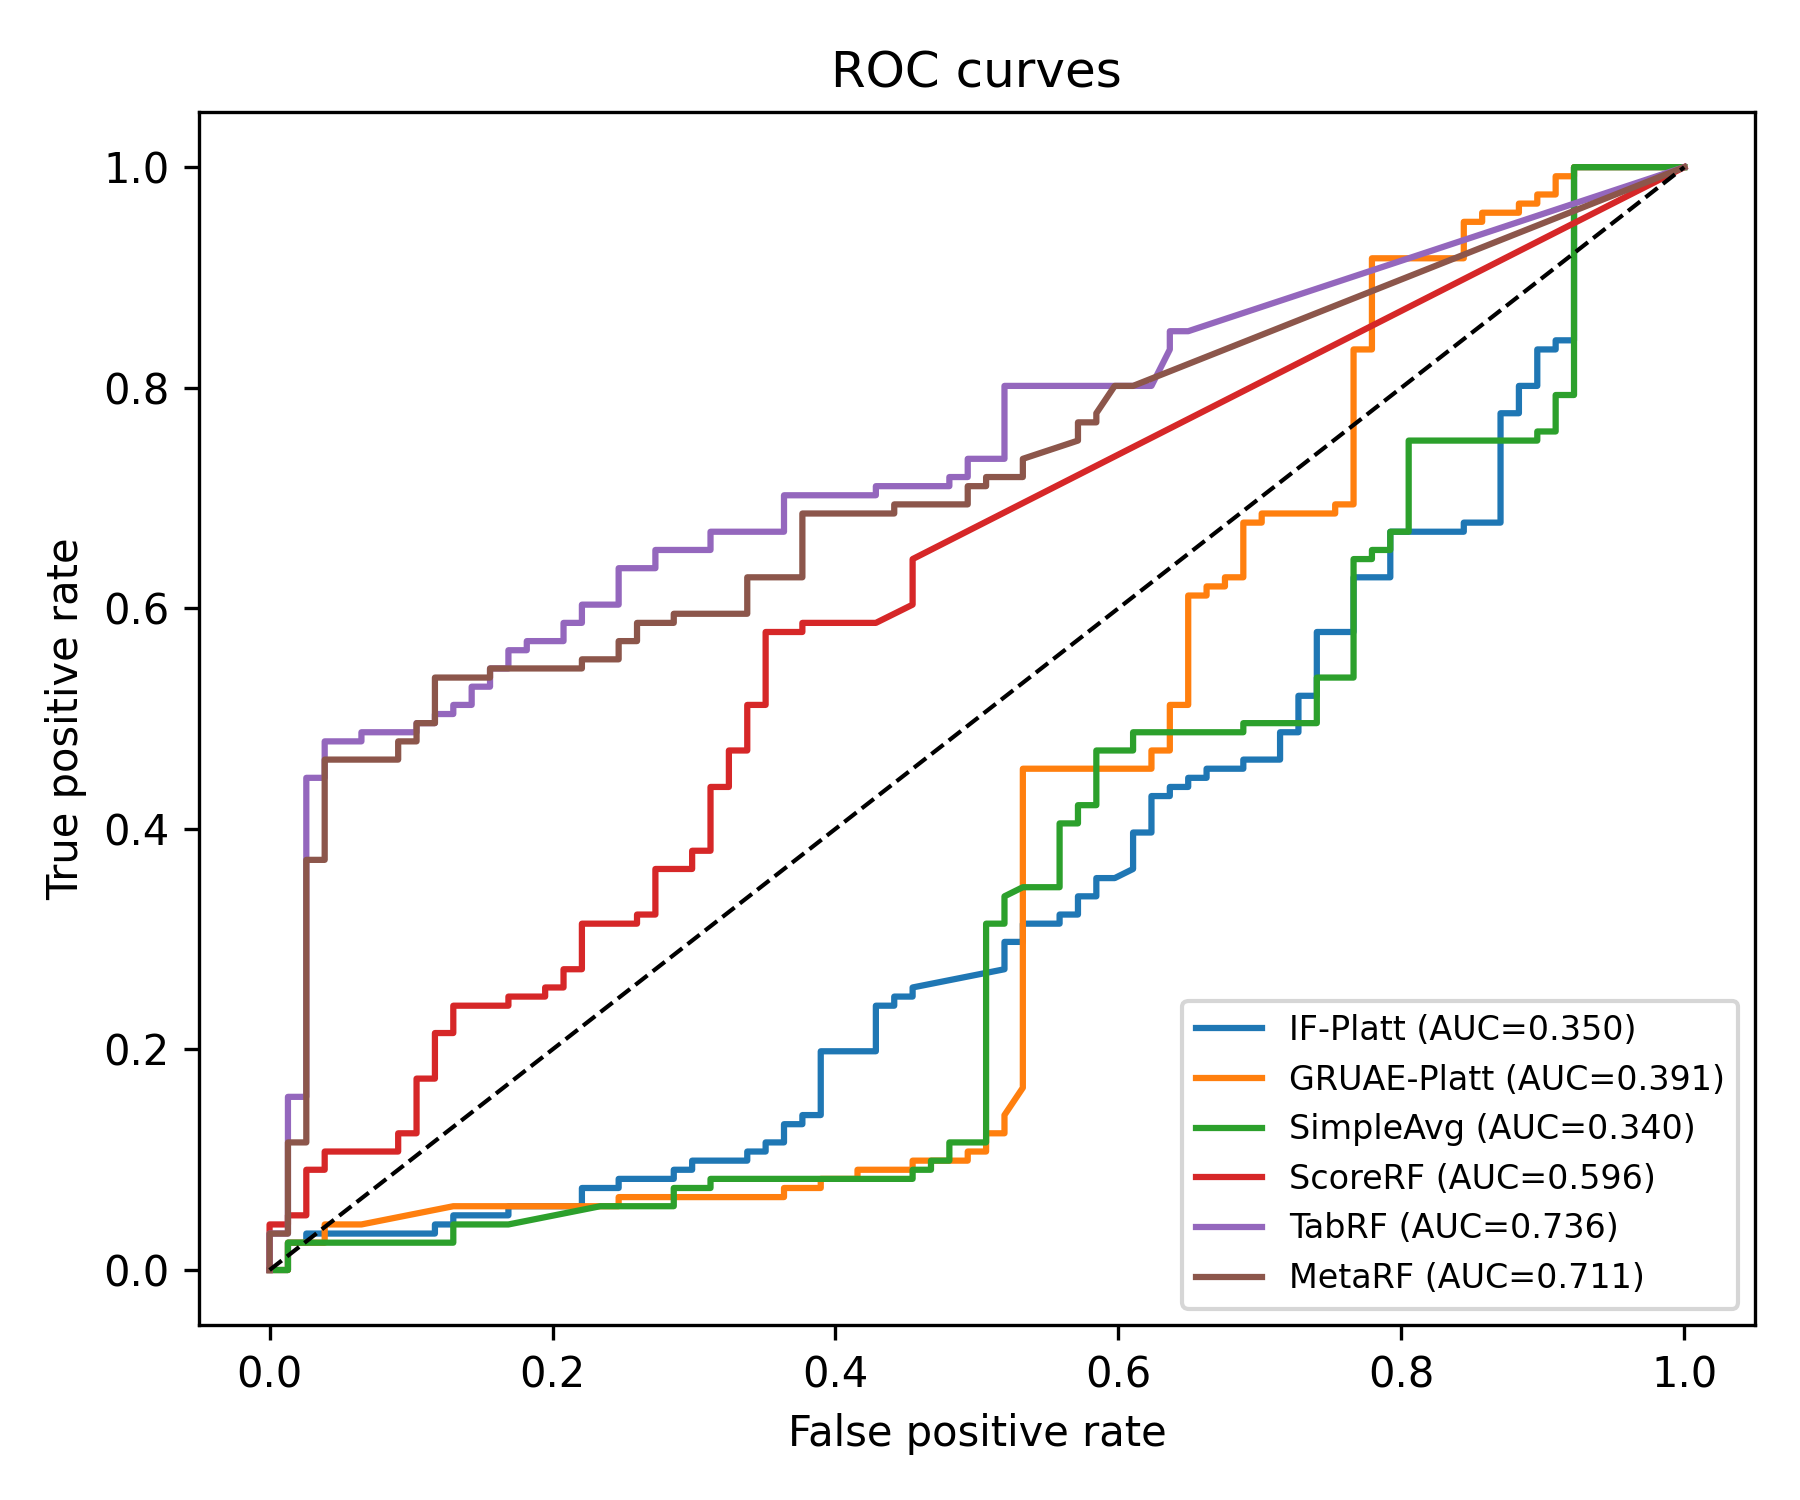
\includegraphics[width=0.95\linewidth]{roc_curves.png}
\caption{ROC curves on the official BETH test split. The tabular and meta Random Forests have stronger ranking behavior than the raw detector scores.}
\label{fig:roc}
\end{figure}

\begin{figure}[t]
\centering
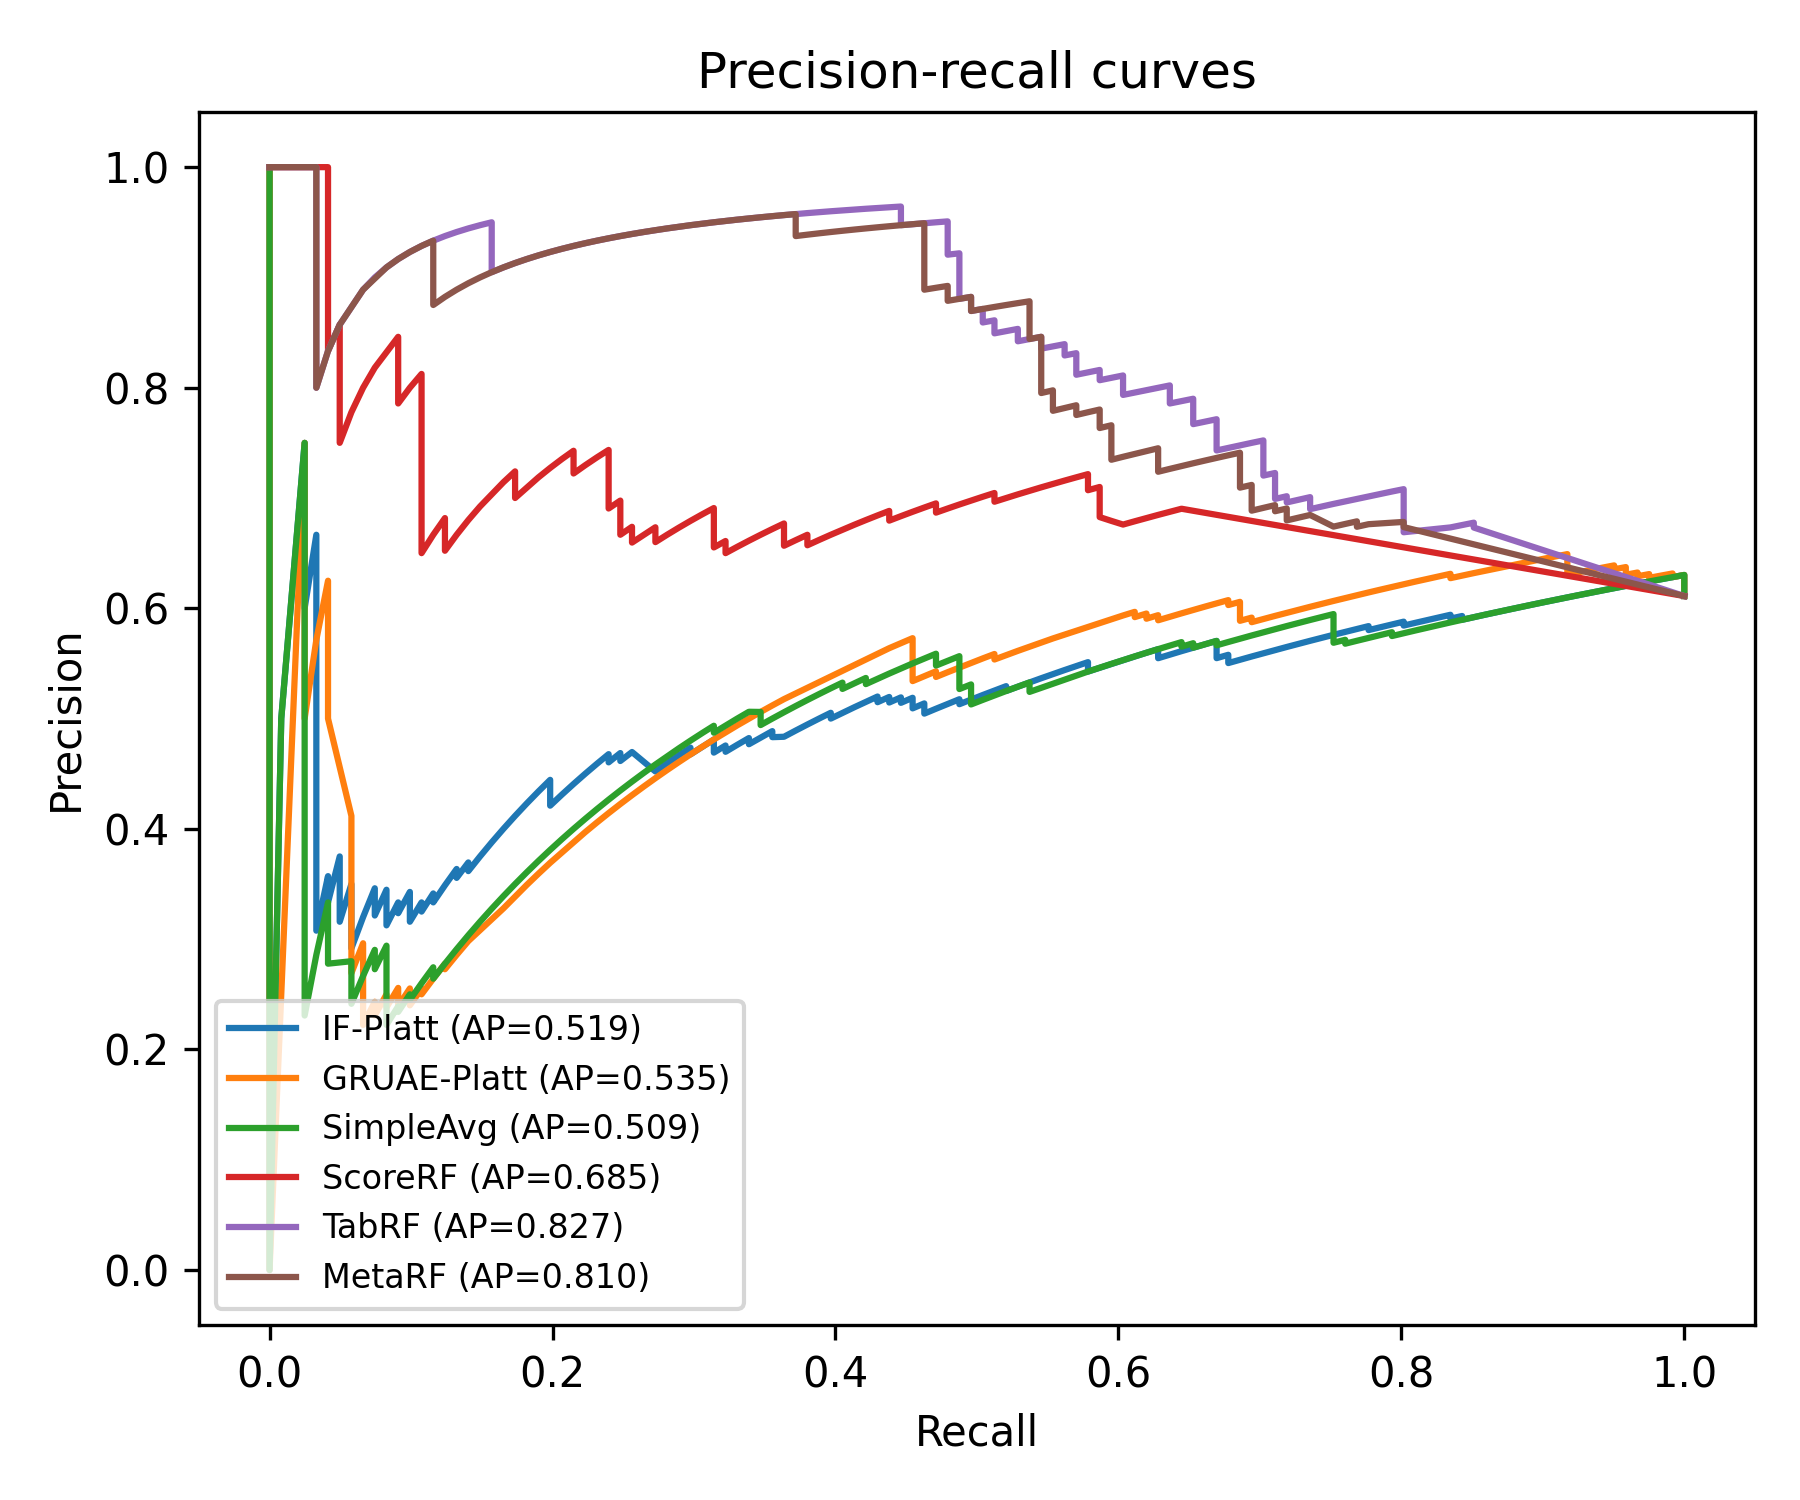
\includegraphics[width=0.95\linewidth]{pr_curves.png}
\caption{Precision-recall curves on the official BETH test split. AP is reported in the legend of the generated figure.}
\label{fig:pr}
\end{figure}

\begin{figure*}[t]
\centering
\subfloat[ScoreRF]{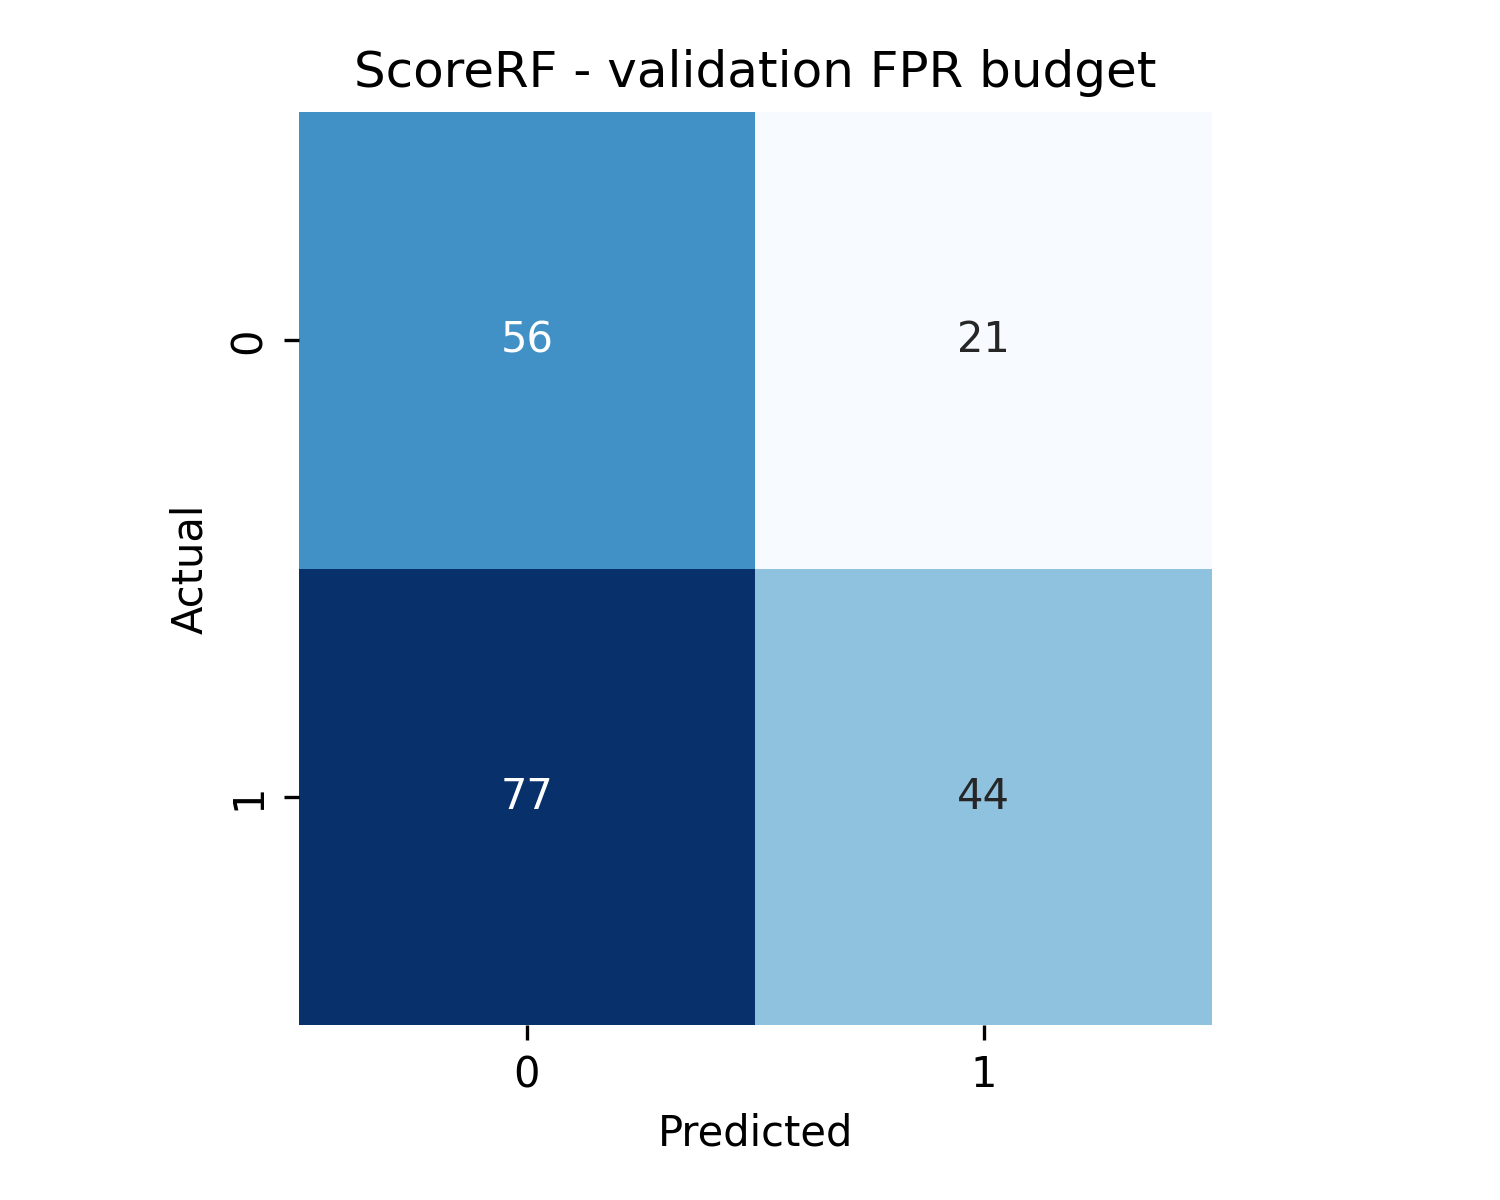
\includegraphics[width=0.31\linewidth]{cm_scorerf_budget.png}}
\hfill
\subfloat[TabRF]{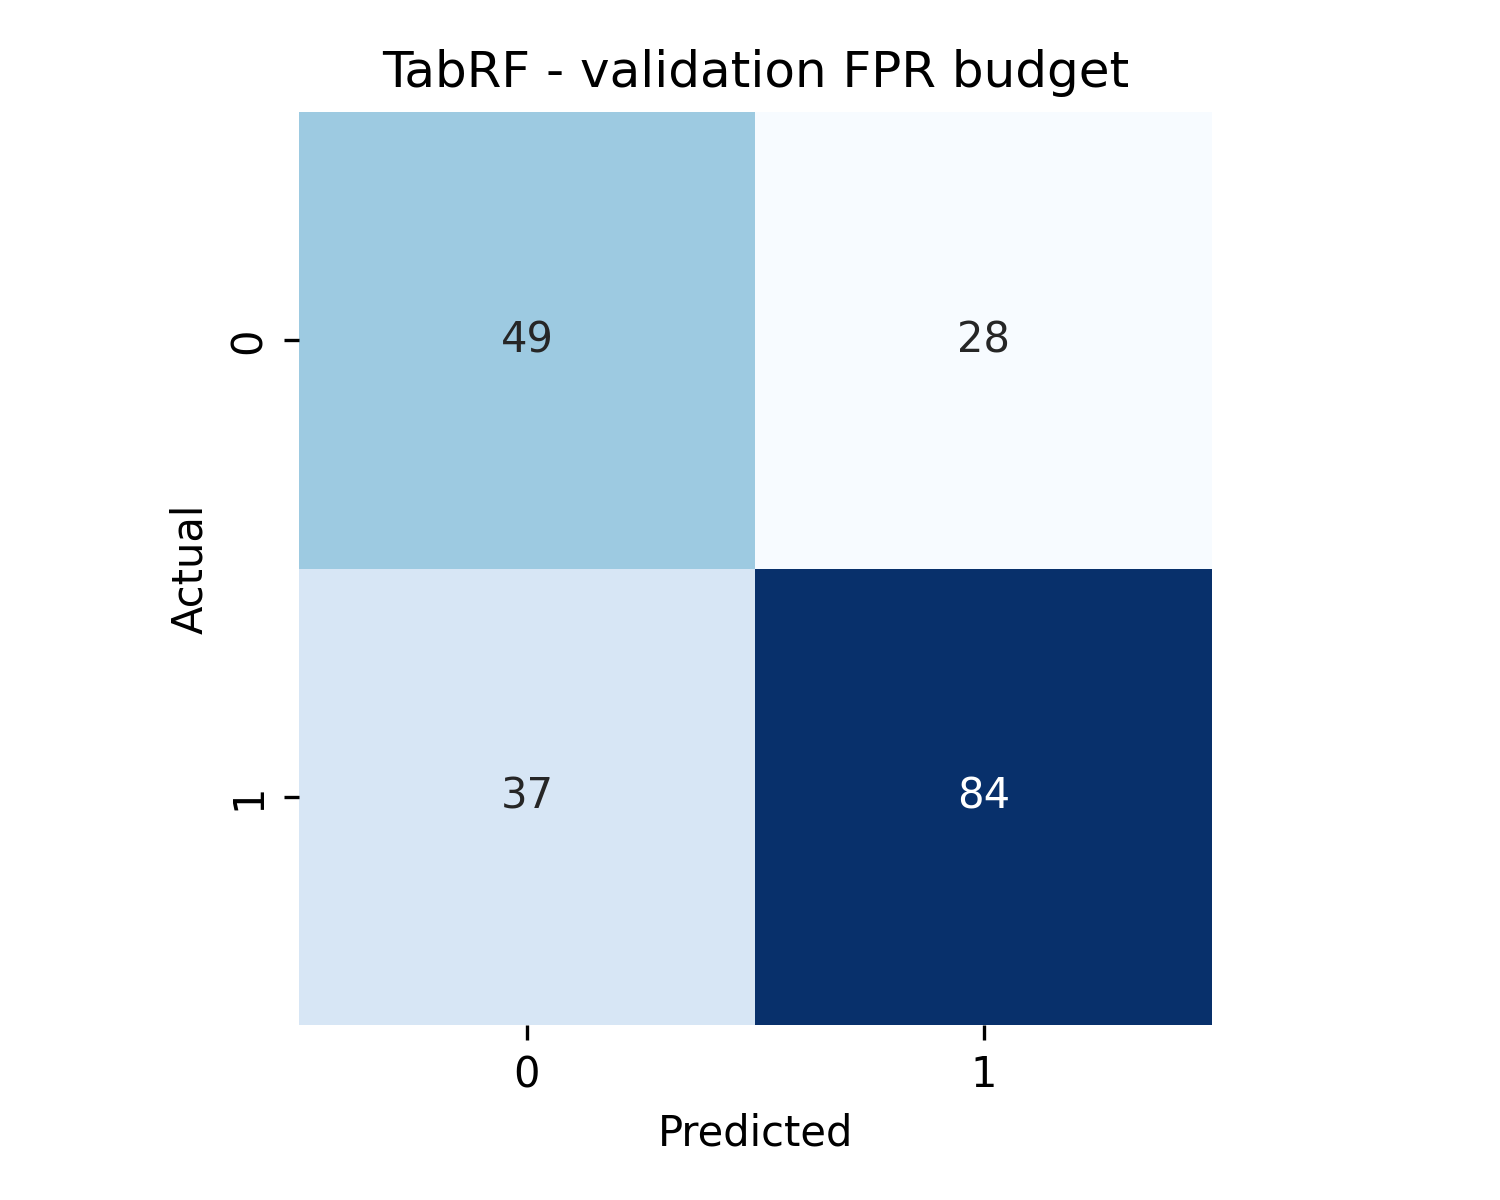
\includegraphics[width=0.31\linewidth]{cm_tabrf_budget.png}}
\hfill
\subfloat[MetaRF]{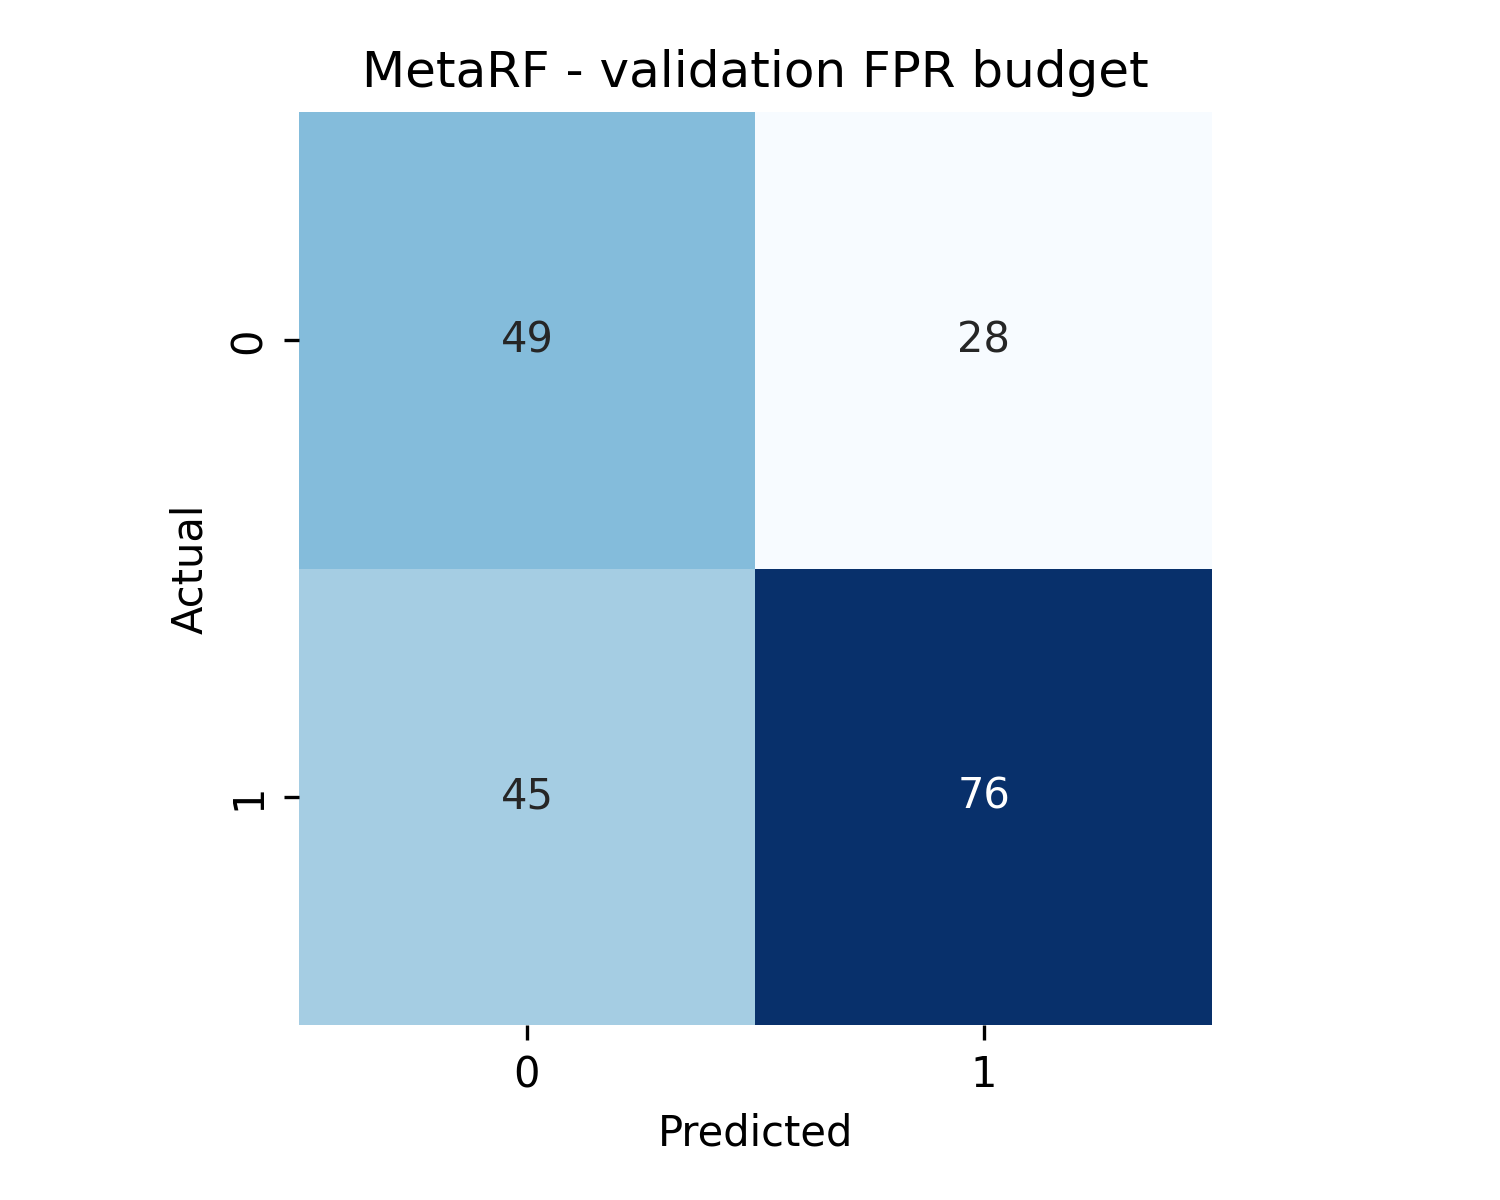
\includegraphics[width=0.31\linewidth]{cm_metarf_budget.png}}
\caption{Confusion matrices under the validation-FPR budget policy. TabRF detects the most malicious processes while maintaining the same false-positive count as MetaRF.}
\label{fig:cms}
\end{figure*}

\subsection{Effect of Threshold Policy}

The validation-max-F1 policy behaves differently from the validation-FPR policy. For TabRF, max-F1 on validation selects a much higher threshold, yielding precision 0.9583 but recall 0.3802 and F1 0.5444 on test. For MetaRF, the corresponding threshold yields precision 0.9474 but recall 0.2975 and F1 0.4528. Thus, optimizing F1 on a validation set with four positives does not generalize to the official test split.

This is a practical lesson: a validation set can be stratified but still too small to support stable threshold optimization. A threshold policy based on a false-positive budget is easier to justify operationally, but it also fails to preserve the target FPR under severe distribution shift. In the present experiment, the threshold is not wrong in a procedural sense; it is wrong because the validation distribution is not representative of the test distribution.

\subsection{Calibration Audit}

Table~\ref{tab:calibration_audit} reports expected calibration error and Brier score on the official test split for the supervised tabular models. Figure~\ref{fig:reliability} gives the corresponding reliability diagrams. ECE values near 0.50 indicate near-null calibration: calibrated scores carry no reliable probability interpretation on the BETH test distribution. TabRF has ECE 0.4984 and Brier score 0.4506, while MetaRF has ECE 0.5007 and Brier score 0.4621. Platt scaling normalizes score ranges but does not produce meaningful posterior estimates under this prevalence mismatch. Logistic regression has the lowest ECE among the audited models (0.2905), but its validation-FPR F1 is only 0.1739. Calibration quality and operational detection quality therefore diverge, and the final claims treat model outputs as scores for thresholding rather than reliable posterior probabilities.

\begin{table}[t]
\centering
\caption{Calibration audit on the official BETH test split. Lower ECE and Brier scores indicate better calibration, but these values should be read together with thresholded detection performance.}
\label{tab:calibration_audit}
\begin{tabular}{lcc}
\toprule
\textbf{Model} & \textbf{ECE} & \textbf{Brier} \\
\midrule
LogReg & 0.2905 & 0.2734 \\
XGBoost & 0.3876 & 0.3725 \\
ExtraTrees & 0.3932 & 0.3498 \\
RF-500 & 0.4924 & 0.4475 \\
TabRF & 0.4984 & 0.4506 \\
MetaRF & 0.5007 & 0.4621 \\
GradientBoosting & 0.5029 & 0.4980 \\
HistGradientBoosting & 0.5177 & 0.5124 \\
ScoreRF & 0.5378 & 0.5243 \\
MLP & 0.5913 & 0.5782 \\
\bottomrule
\end{tabular}
\end{table}

\begin{figure*}[t]
\centering
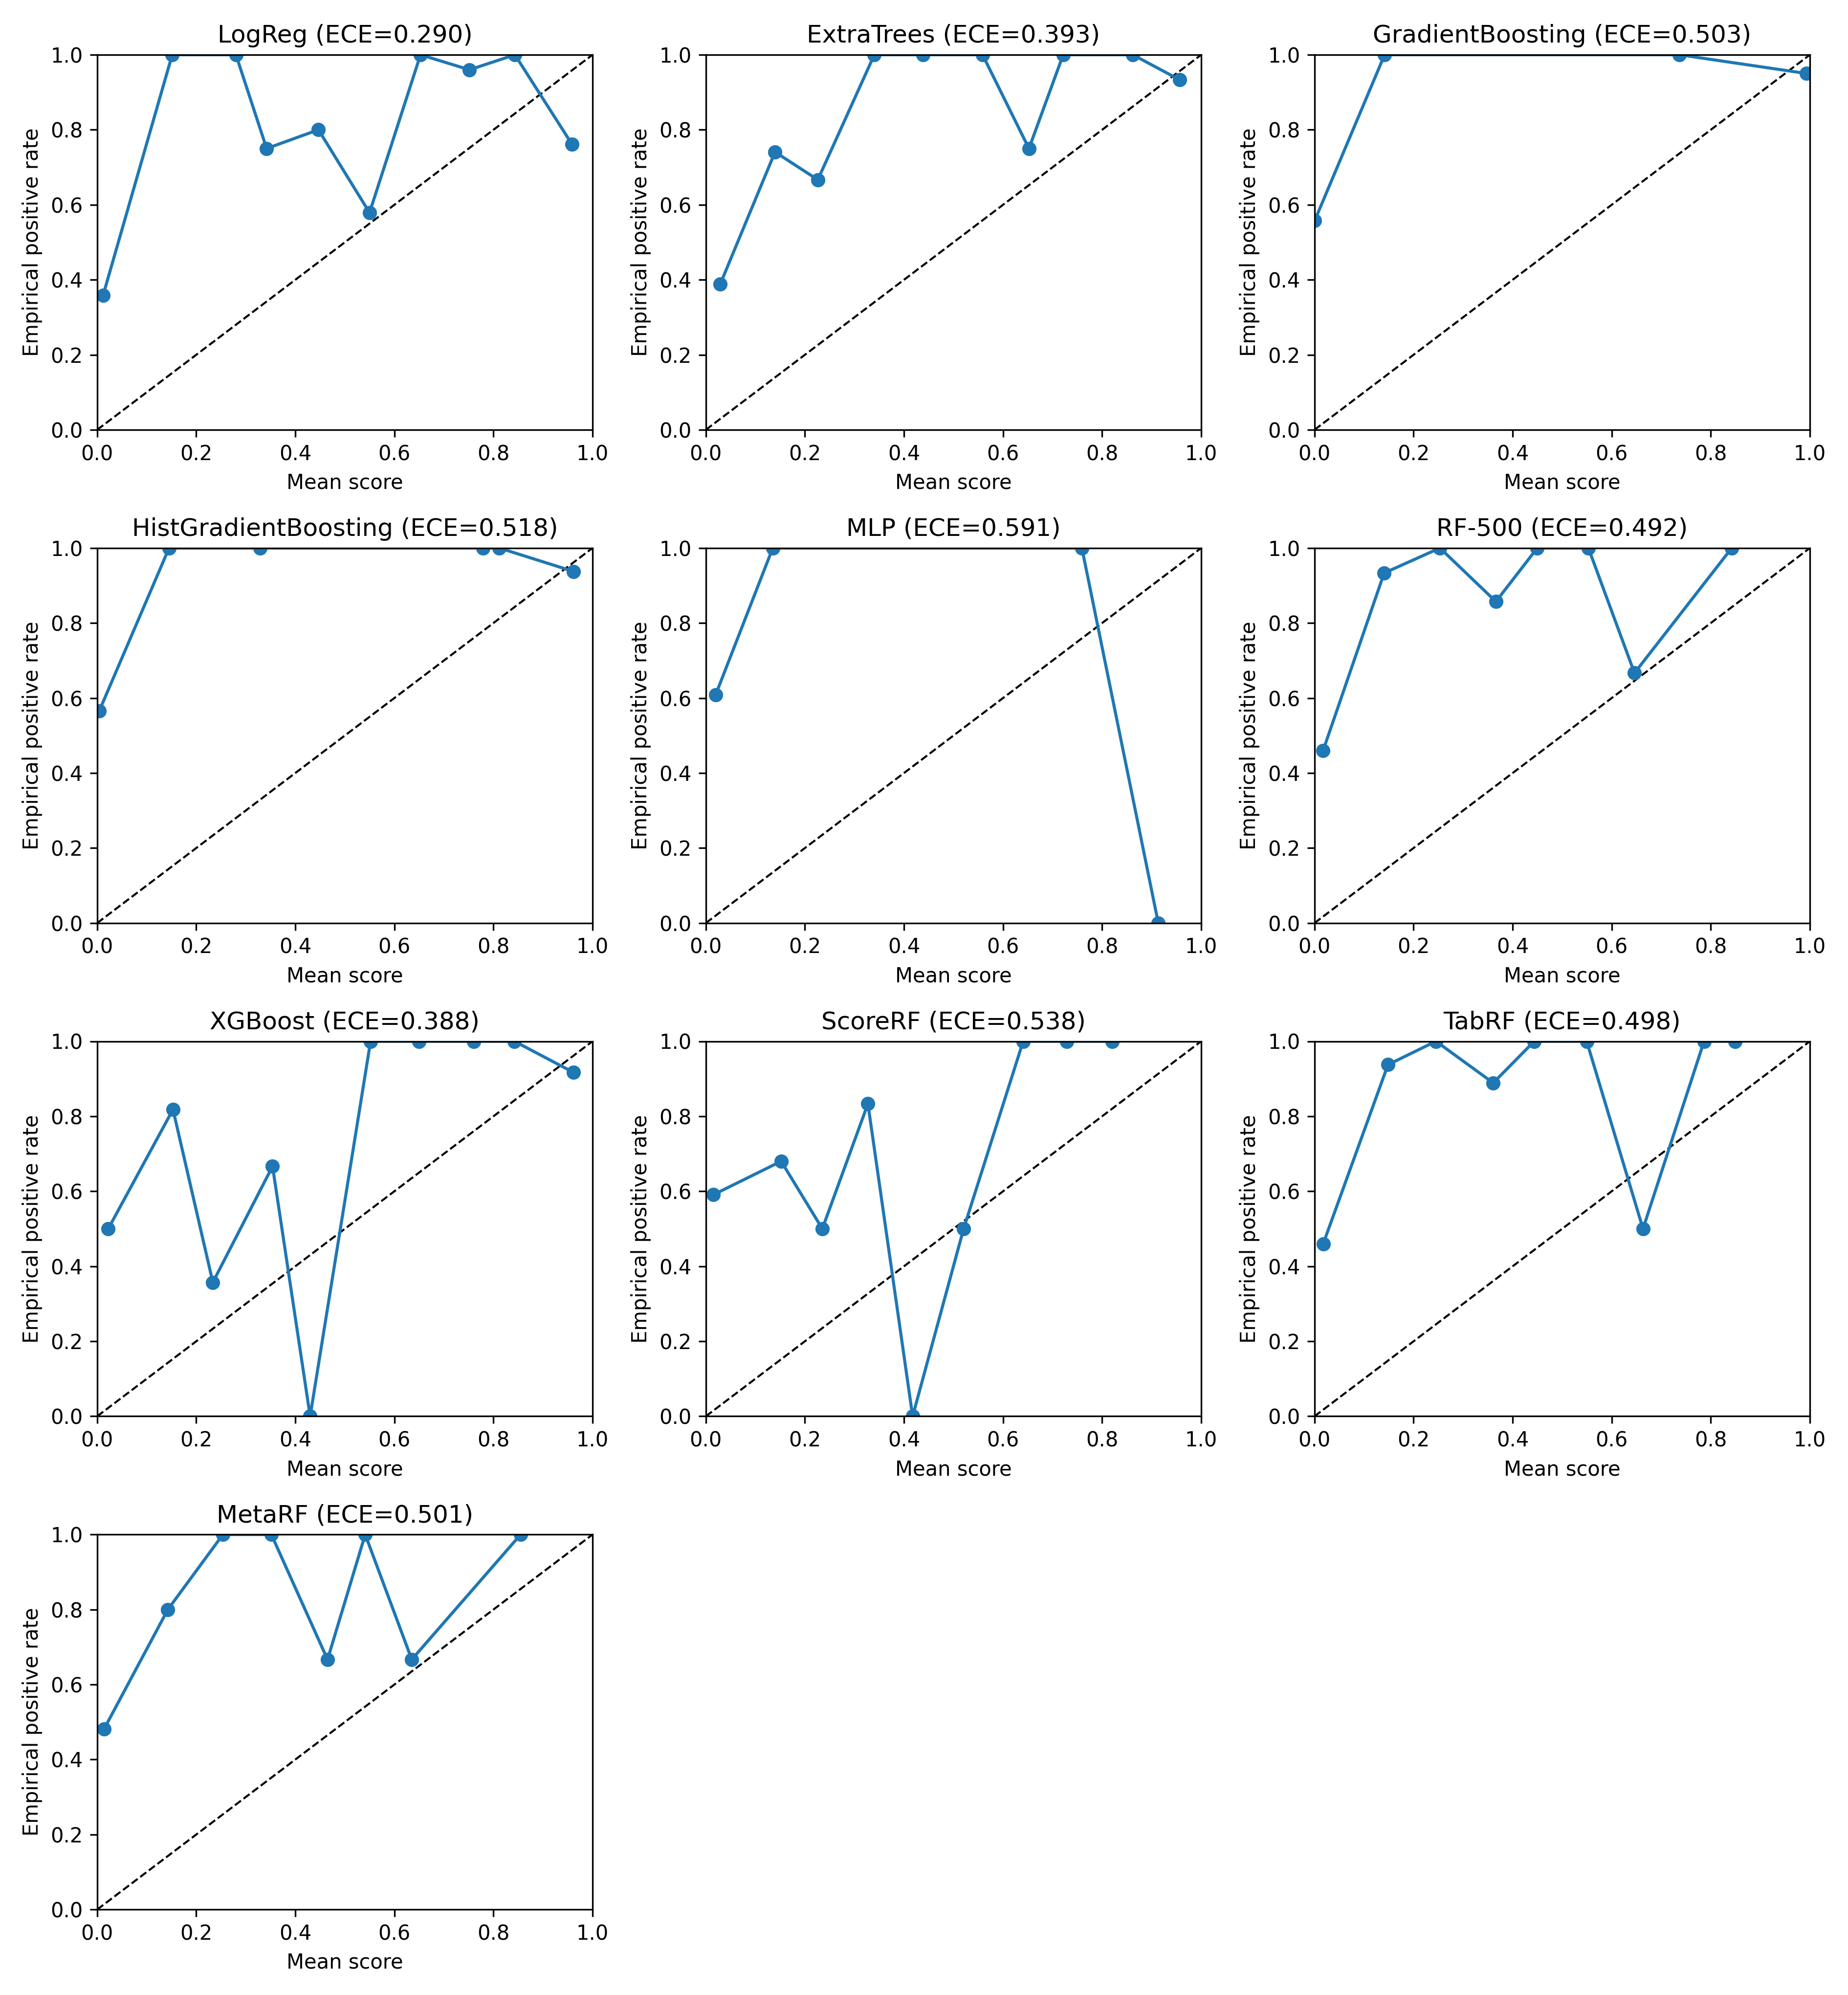
\includegraphics[width=0.95\textwidth]{reliability_diagrams.png}
\caption{Reliability diagrams for the additional tabular audit on the official BETH test split. The diagrams support the paper's use of score and threshold language rather than calibrated-risk language.}
\label{fig:reliability}
\end{figure*}

\subsection{Ablation Interpretation}

The ablation structure isolates three information levels:
\begin{itemize}
    \item calibrated anomaly scores only (ScoreRF);
    \item raw aggregated behavioral features only (TabRF);
    \item raw features plus calibrated scores (MetaRF).
\end{itemize}
ScoreRF has F1 0.4731 under the main policy. This means the two detector scores contain some signal, but not enough. RF-500 and TabRF reach F1 0.7241 and 0.7210, indicating that the event histogram and scalar process features are the dominant source of predictive information. MetaRF has F1 0.6756, showing that adding score features does not improve the Random Forest. The likely reason is redundancy: the Isolation Forest and GRU-AE scores are derived from the same event and sequence information already available to the supervised tree ensemble, but in a compressed form that loses discriminative detail.

\subsection{Why the Individual Detectors Invert}

The Isolation Forest has AUC 0.3496 and the GRU-AE has AUC 0.3913. AUC below 0.5 means the score ordering is partially inverted: many malicious test processes receive lower anomaly scores than benign test processes. This can happen when the benign development distribution contains long, diverse, or noisy processes that look more anomalous than the malicious processes in the official test split. It can also occur if malicious test traces are internally consistent and therefore reconstructed well by a sequence model trained on benign event syntax.

This inversion is not a software bug by itself. It is an empirical property of the representation and split. It does, however, weaken any claim that unsupervised anomaly detection alone is sufficient for BETH process-level malicious-process detection.

\section{External Validation on MalBehavD-V1}
\label{sec:external_malbehavd}

To test whether FAIR-BETH is useful beyond BETH, we apply the same evaluation principles to MalBehavD-V1 \cite{maniriho2023,malbehavd2023}, an independent dynamic Windows malware dataset. MalBehavD-V1 contains API-call sequences extracted from benign and malware executables executed in a Cuckoo sandbox. The public CSV used here contains 2\,570 samples: 1\,285 benign files and 1\,285 malware files. Sequence length ranges from 2 to 175 API calls, with median length 37 and 291 unique API names.

The external experiment is not a direct transfer of the BETH-trained TabRF model. Direct transfer would be invalid because BETH contains endpoint event records, while MalBehavD-V1 contains ordered Windows API-call sequences. Instead, the purpose is protocol validation: the same FAIR-BETH rules are applied to an independent behavioral dataset. Labels are excluded from predictors; feature vocabularies are fit only on training data; thresholds are selected only on validation data; and oracle test thresholds are reported only as non-deployable upper bounds.

We represent each API-call sequence by scalar sequence statistics, API-family rates, and normalized API histograms using the 128 most frequent training APIs. The Random Forest uses 300 trees, balanced class weights, and minimum leaf size 2. The fixed split allocates 60\% of the data to training, 15\% to calibration, 10\% to validation, and 15\% to testing. We also run 30 repeated stratified splits to estimate split sensitivity.

\begin{table*}[t]
\centering
\caption{External validation on MalBehavD-V1 using full API-call sequences. The oracle threshold is shown only as a non-deployable upper bound.}
\label{tab:malbehavd_external}
\begin{tabular}{lcccccccc}
\toprule
\textbf{Threshold policy} & \textbf{AUC} & \textbf{AP} & \textbf{Precision} & \textbf{Recall} & \textbf{F1} & \textbf{F1 95\% CI} & \textbf{FP} & \textbf{FN} \\
\midrule
Validation-FPR budget & 0.9902 & 0.9922 & 0.9439 & 0.9585 & 0.9512 & [0.9291, 0.9720] & 11 & 8 \\
Validation-max-F1 & 0.9902 & 0.9922 & 0.9735 & 0.9534 & 0.9634 & [0.9430, 0.9809] & 5 & 9 \\
Oracle test max-F1 & 0.9902 & 0.9922 & 0.9737 & 0.9585 & 0.9661 & [0.9468, 0.9834] & 5 & 8 \\
\bottomrule
\end{tabular}
\end{table*}

Table~\ref{tab:malbehavd_external} shows that the FAIR-BETH protocol is not tied to BETH-specific artifacts. Under a validation-FPR threshold, the external Random Forest reaches F1 0.9512 with 11 false positives and 8 false negatives on the held-out test split. The oracle threshold improves F1 only slightly, from 0.9512 to 0.9661. This small oracle gap is important: unlike BETH, where threshold transfer is fragile, MalBehavD-V1 has enough balanced validation signal for threshold selection to behave more stably.

Across 30 repeated stratified splits under the validation-FPR policy, mean F1 is 0.9530, median F1 is 0.9533, and the interquartile range is [0.9429, 0.9634]. Mean AUC is 0.9869 and mean AP is 0.9902. These repeated-split results show that the external result is not a single favorable split.

\begin{table}[t]
\centering
\caption{Prefix-length evaluation on MalBehavD-V1 under the validation-FPR threshold policy.}
\label{tab:malbehavd_prefix}
\begin{tabular}{lcccc}
\toprule
\textbf{API prefix} & \textbf{AUC} & \textbf{Precision} & \textbf{Recall} & \textbf{F1} \\
\midrule
10 calls & 0.9672 & 0.9494 & 0.8756 & 0.9111 \\
25 calls & 0.9813 & 0.9775 & 0.9016 & 0.9380 \\
50 calls & 0.9877 & 0.9780 & 0.9223 & 0.9493 \\
100 calls & 0.9905 & 0.9538 & 0.9637 & 0.9588 \\
Full sequence & 0.9902 & 0.9439 & 0.9585 & 0.9512 \\
\bottomrule
\end{tabular}
\end{table}

Table~\ref{tab:malbehavd_prefix} and Figure~\ref{fig:malbehavd_prefix} address the early-detection limitation. With only the first 10 API calls, the model already reaches F1 0.9111. Performance improves with longer prefixes, and the 100-call prefix slightly exceeds the full-sequence F1 under the validation-FPR policy. This does not prove real-time ransomware containment, but it shows how FAIR-BETH can be extended from full-trace classification to prefix-based behavioral detection.

\begin{figure}[t]
\centering
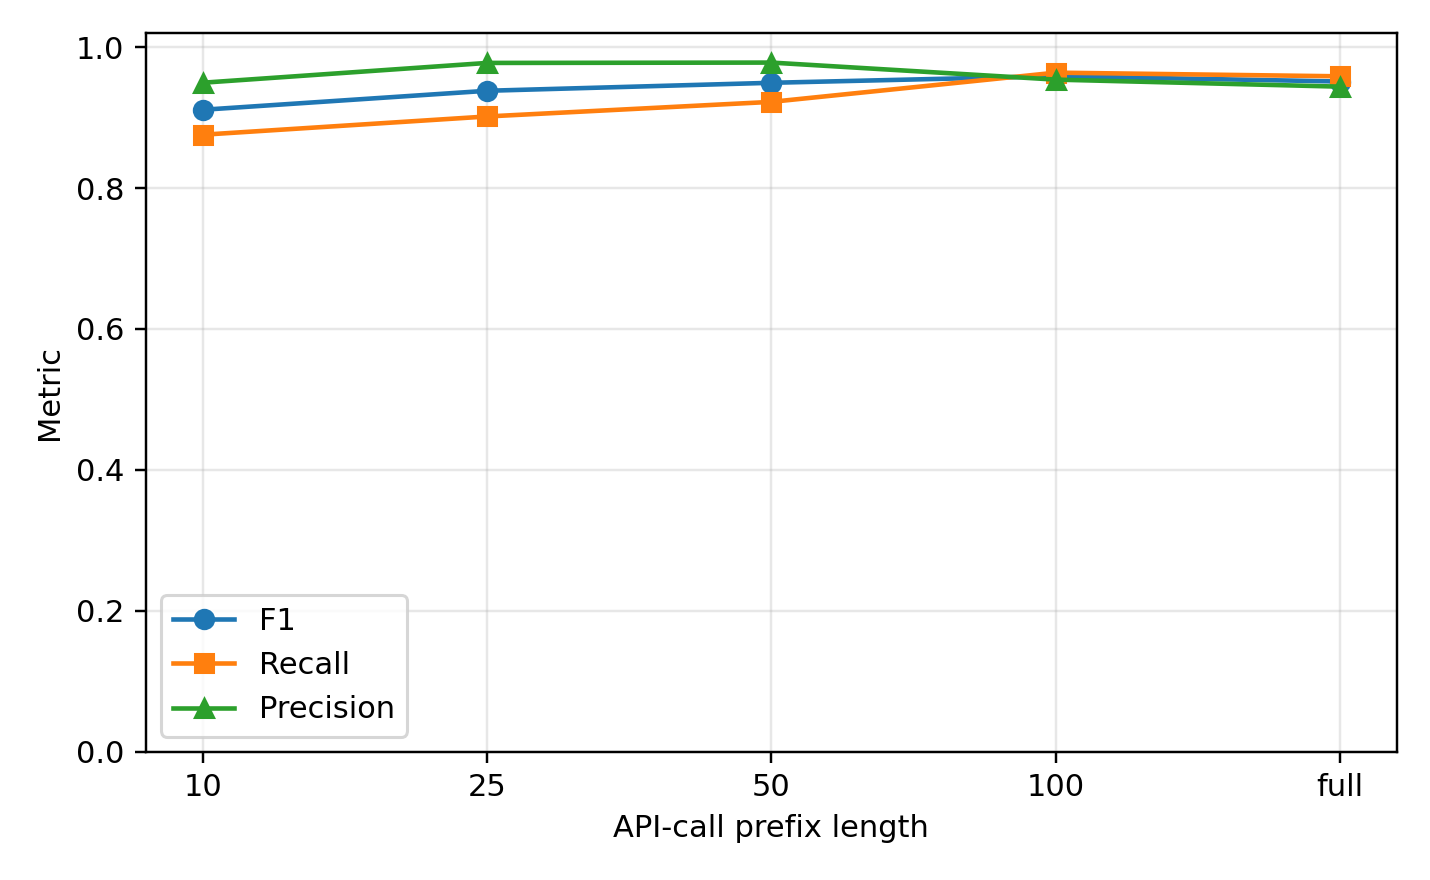
\includegraphics[width=0.95\linewidth]{malbehavd_prefix_curve.png}
\caption{MalBehavD-V1 prefix evaluation. The curve shows that useful discrimination is available before the full API-call sequence is observed.}
\label{fig:malbehavd_prefix}
\end{figure}

Finally, Figure~\ref{fig:malbehavd_importance} reports permutation feature attribution on the fixed external test split. The highest-ranked features are API-specific and family-rate features derived only after final evaluation. They are not used to tune the model. This preserves the separation between model selection and interpretation.

\begin{figure}[t]
\centering
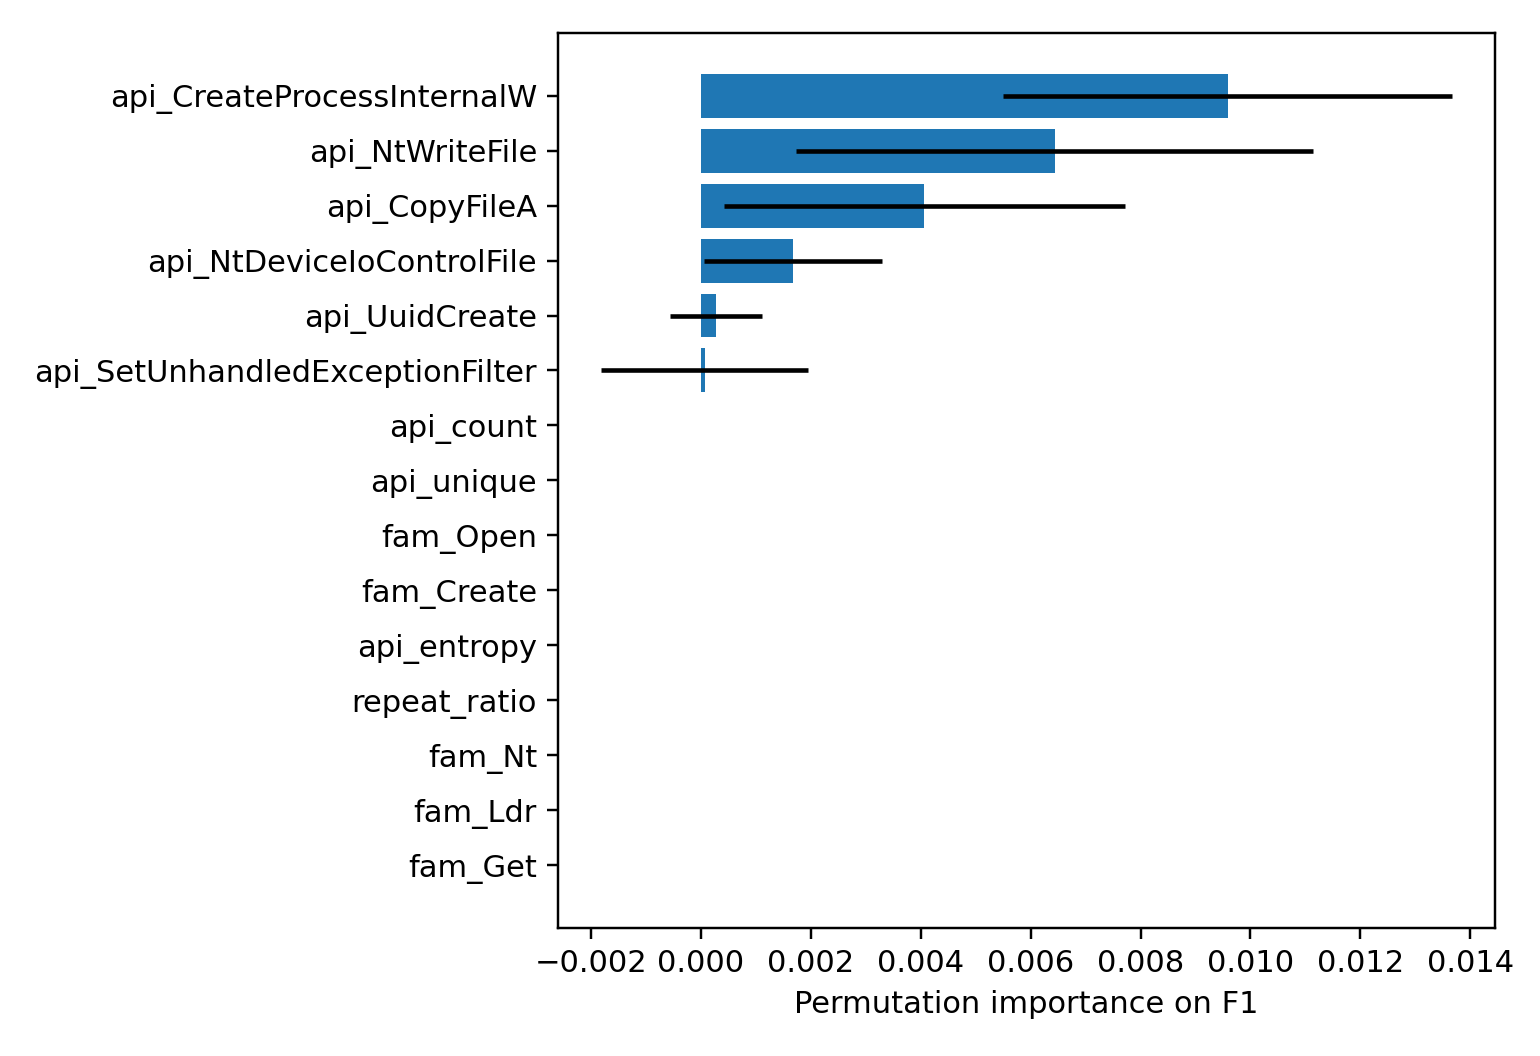
\includegraphics[width=0.95\linewidth]{malbehavd_feature_importance.png}
\caption{Permutation feature importance on MalBehavD-V1. Attribution is computed after final evaluation and is used only for interpretation.}
\label{fig:malbehavd_importance}
\end{figure}

\section{Additional Limit-Lifting Audits on BETH}
\label{sec:limit_lifting}

The external MalBehavD-V1 experiment tests whether the evaluation protocol transfers to a second behavioral schema. We also add five BETH-specific audits to reduce remaining ambiguity: feature attribution, prefix detection, cost-sensitive thresholding, feature-space stress testing, and host/temporal split robustness. These audits use the already selected TabRF model unless stated otherwise. They are not used to tune the main result.

Figure~\ref{fig:beth_importance} reports held-out permutation importance for TabRF on the official BETH test split. The dominant predictors are eventId histogram features, event entropy, process size, duration, event rate, and argument diversity. This supports the interpretation that TabRF is not relying on label annotations or ATT\&CK-derived predictors; it is using observable behavioral composition and process-scale statistics.

\begin{figure}[t]
\centering
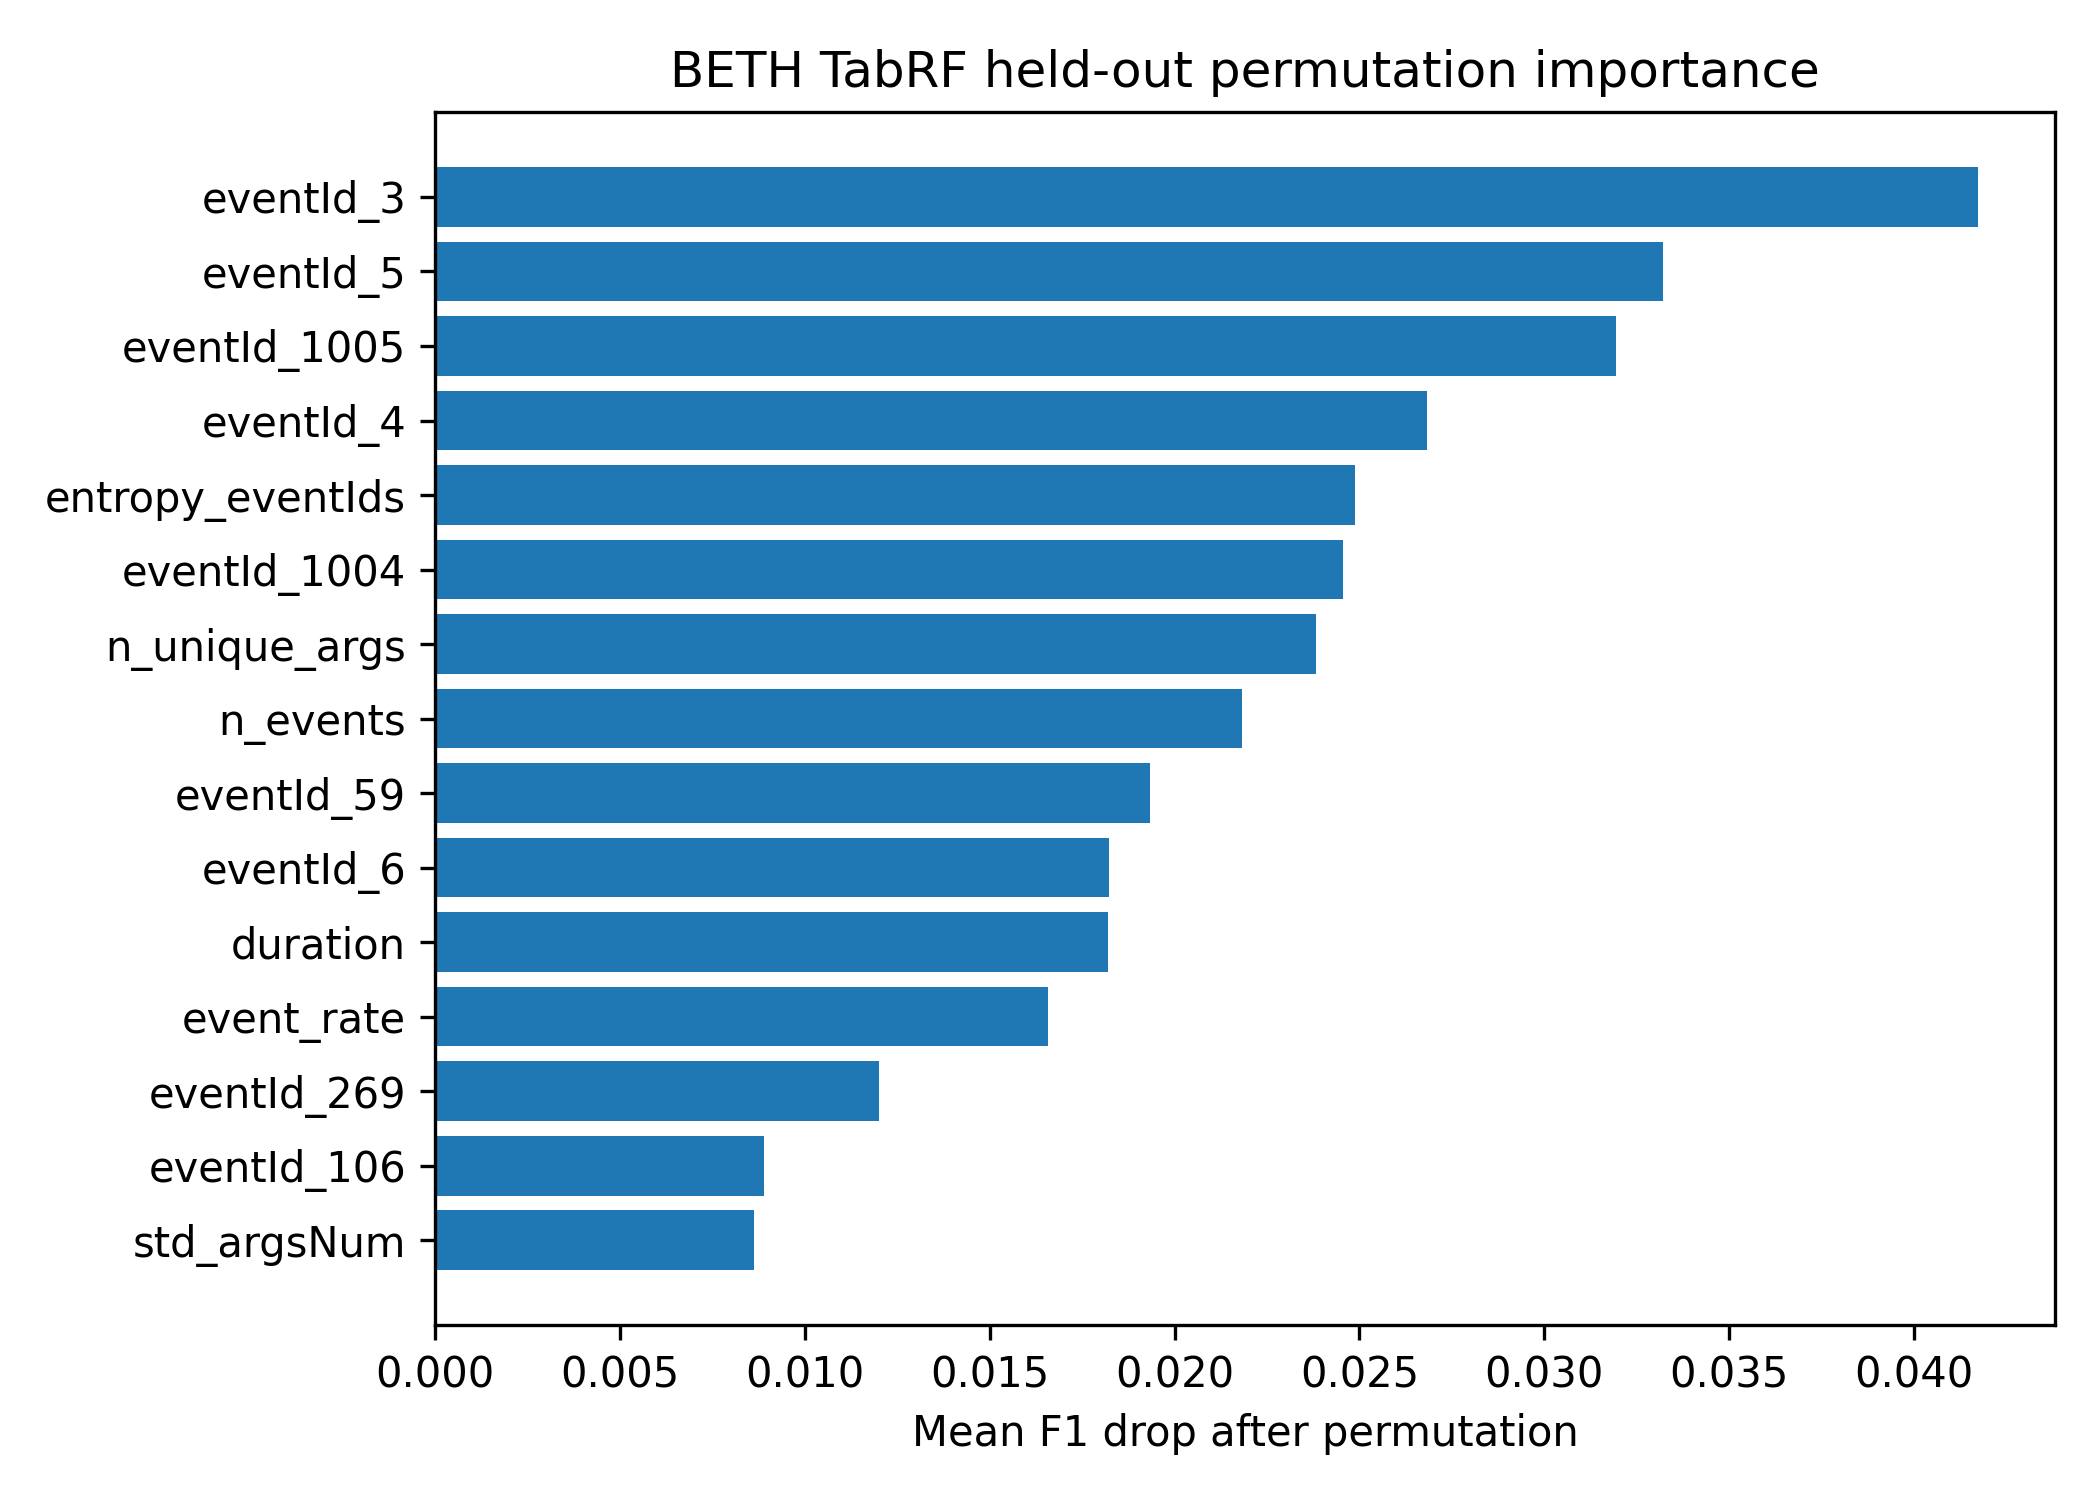
\includegraphics[width=0.95\linewidth]{beth_tabrf_permutation_importance.png}
\caption{Held-out permutation importance for BETH TabRF on the official test split. Importance is computed after final evaluation and is not used for tuning.}
\label{fig:beth_importance}
\end{figure}

Table~\ref{tab:beth_prefix} and Figure~\ref{fig:beth_prefix} evaluate TabRF on prefixes of BETH process traces. The validation-FPR threshold is reselected on the corresponding validation prefix. The result is materially weaker than full-trace classification: F1 is 0.0775 after 10 events, 0.3576 after 25 events, 0.5349 after 250 events, and 0.7210 only when the full process trace is available. This directly addresses the latency limitation. On BETH, the current full-process representation should not be claimed as an early containment detector.

\begin{table}[t]
\centering
\caption{BETH TabRF prefix evaluation under validation-FPR thresholding.}
\label{tab:beth_prefix}
\begin{tabular}{lcccc}
\toprule
\textbf{Prefix} & \textbf{AUC} & \textbf{Prec.} & \textbf{Rec.} & \textbf{F1} \\
\midrule
10 events & 0.4443 & 0.6250 & 0.0413 & 0.0775 \\
25 events & 0.5553 & 0.9000 & 0.2231 & 0.3576 \\
50 events & 0.6678 & 0.8500 & 0.2810 & 0.4224 \\
100 events & 0.6414 & 0.7857 & 0.3636 & 0.4972 \\
250 events & 0.6572 & 0.9020 & 0.3802 & 0.5349 \\
Full trace & 0.7360 & 0.7500 & 0.6942 & 0.7210 \\
\bottomrule
\end{tabular}
\end{table}

\begin{figure}[t]
\centering
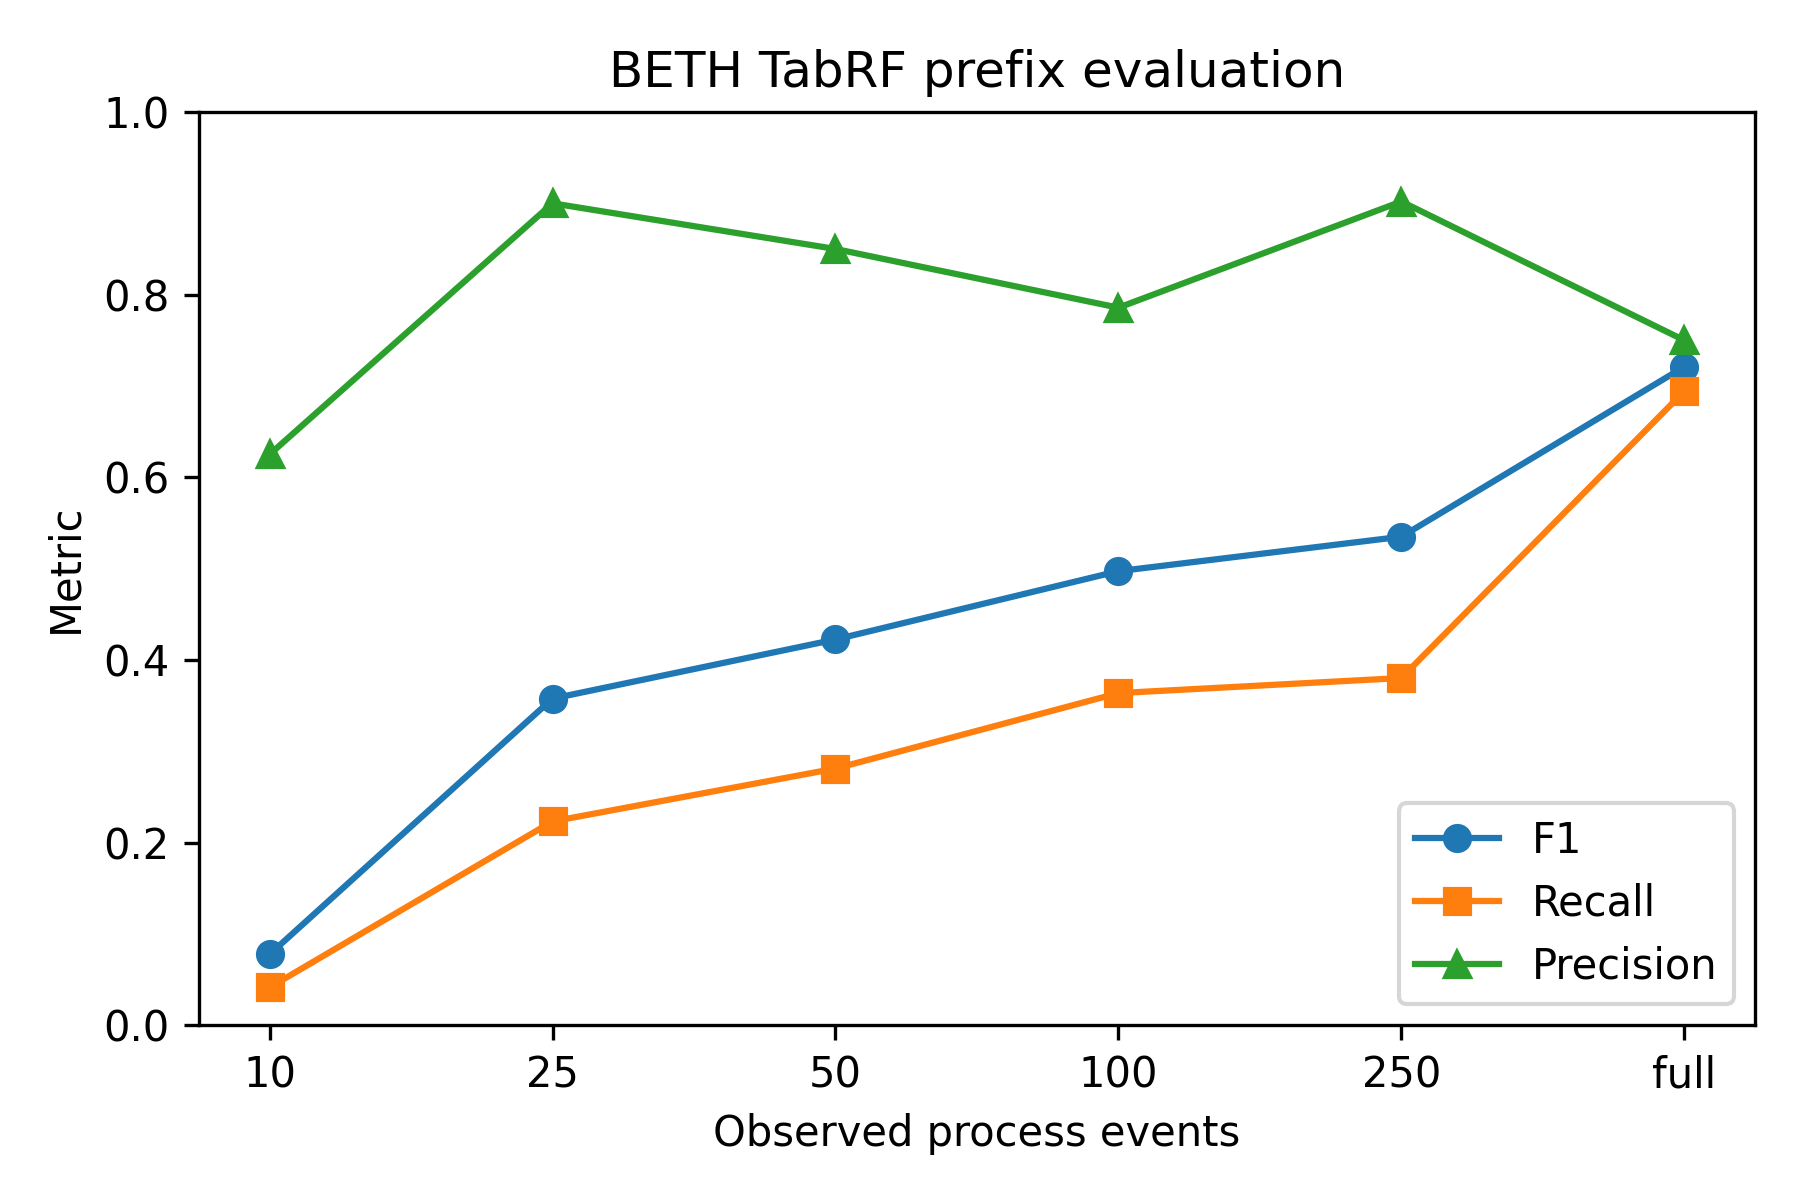
\includegraphics[width=0.95\linewidth]{beth_prefix_curve.png}
\caption{BETH TabRF prefix curve. Unlike MalBehavD-V1, BETH requires much more of the process trace before recall becomes useful.}
\label{fig:beth_prefix}
\end{figure}

Table~\ref{tab:beth_cost} replaces a single F1 operating point with explicit cost assumptions. When false negatives and false positives have equal cost, the lowest empirical cost occurs at threshold 0.0274, with 21 false positives and 42 false negatives. When a false negative costs at least five times a false positive, the cost-minimizing threshold on this test split is zero, producing no false negatives but 77 false positives. This is not a deployable recommendation, because it uses test labels to illustrate cost sensitivity. It shows that response policy cannot be inferred from F1 alone.

\begin{table}[t]
\centering
\caption{BETH TabRF cost-sensitive threshold audit on the official test split. Thresholds are oracle cost minima and are reported only to expose cost sensitivity.}
\label{tab:beth_cost}
\begin{tabular}{ccccc}
\toprule
\textbf{FN:FP} & \textbf{Thr.} & \textbf{FP} & \textbf{FN} & \textbf{F1} \\
\midrule
1:1 & 0.0274 & 21 & 42 & 0.7149 \\
5:1 & 0.0000 & 77 & 0 & 0.7586 \\
10:1 & 0.0000 & 77 & 0 & 0.7586 \\
25:1 & 0.0000 & 77 & 0 & 0.7586 \\
50:1 & 0.0000 & 77 & 0 & 0.7586 \\
\bottomrule
\end{tabular}
\end{table}

Table~\ref{tab:beth_stress} reports simple feature-space stress tests at the original validation-FPR threshold. Event-histogram dropout and malicious slowdown do not collapse the detector, but they change precision, recall, and ranking. These tests are not a substitute for malware-level evasion experiments; they are a concrete lower-bound audit showing how the trained model reacts when behavioral composition or event timing is perturbed.

\begin{table}[t]
\centering
\caption{BETH TabRF feature-space stress tests at the original validation-FPR threshold.}
\label{tab:beth_stress}
\begin{tabular}{lccc}
\toprule
\textbf{Stress test} & \textbf{AUC} & \textbf{Recall} & \textbf{F1} \\
\midrule
None & 0.7360 & 0.6942 & 0.7210 \\
10\% event dropout & 0.7334 & 0.7355 & 0.7177 \\
25\% event dropout & 0.6852 & 0.8430 & 0.7312 \\
50\% event dropout & 0.6437 & 0.8843 & 0.7405 \\
Slowdown 0.50 & 0.7341 & 0.6612 & 0.6987 \\
Slowdown 0.25 & 0.7488 & 0.6777 & 0.7100 \\
Slowdown 0.10 & 0.7830 & 0.7521 & 0.7583 \\
\bottomrule
\end{tabular}
\end{table}

Finally, Table~\ref{tab:beth_group_temporal} evaluates group and temporal robustness by retraining TabRF on the enriched development pool under host-disjoint validation splits and a chronological 70/15/15 split, then evaluating once on the official test split. Four of ten host-disjoint validation attempts are skipped because one fold is single-class. Among the six valid host-disjoint folds, median F1 is 0.2739, with range [0.1678, 0.7188]. The chronological split reaches F1 0.4294. This audit partially lifts the split-design limitation by measuring it directly, but it does not eliminate it: positive examples are too concentrated across hosts for host-disjoint threshold selection to be stable.

\begin{table*}[t]
\centering
\caption{BETH split-robustness audit. Host-disjoint results summarize six valid folds; four additional folds were single-class and skipped.}
\label{tab:beth_group_temporal}
\begin{tabular}{lccc}
\toprule
\textbf{Split audit} & \textbf{AUC} & \textbf{Recall} & \textbf{F1} \\
\midrule
Main process split & 0.7360 & 0.6942 & 0.7210 \\
Host-disjoint median & 0.5041 & 0.1860 & 0.2739 \\
Host-disjoint range & 0.4095--0.8300 & 0.0992--0.5702 & 0.1678--0.7188 \\
Temporal 70/15/15 & 0.6865 & 0.2893 & 0.4294 \\
\bottomrule
\end{tabular}
\end{table*}

\section{Protocol Audit}
\label{sec:audit}

\subsection{Leakage Controls}

The first audit question is whether the experiment leaks labels into the predictor. The pipeline avoids the obvious leakage path by excluding \texttt{sus} and \texttt{evil} from feature vectors. These columns are used only to define the process-level target. ATT\&CK mappings are not used as predictors because BETH does not provide technique labels or documented mapping rules for them. The official test file is read during preprocessing to construct test features, but its labels are not used for fitting models, calibration, or threshold selection.

A subtler leakage risk is feature vocabulary construction. If the event vocabulary were fit on train, validation, and test jointly, test-only event identifiers would influence the feature space. The pipeline fits the event vocabulary on the enriched development pool and applies it to test. Unknown test events are handled without expanding the trained feature space. This is important because an event identifier appearing only in the test split could otherwise become a silent test-derived feature.

\subsection{Threshold Fairness}

The second audit question is whether all models receive equivalent threshold treatment. FAIR-BETH evaluates every model under the same validation-derived threshold policies. Under this rule, RF-500 and TabRF at the validation-FPR threshold reach F1 0.7241 and 0.7210, exceeding MetaRF at F1 0.6756. This demonstrates why threshold fairness is not a cosmetic concern; it can determine the interpretation of a hybrid detector.

The paper therefore reports two threshold policies for every model. Neither policy is perfect, but both are applied consistently. This creates a transparent table in which a reader can see how a model behaves under a false-positive constraint and under a validation-F1 objective.

\subsection{Calibration Audit}

The calibration fold contains six malicious processes. This is enough for scikit-learn logistic regression to fit Platt scaling, but it is not enough to trust probability calibration. The Platt-scaled scores are all close to the low development prevalence. The absolute thresholds in Table~\ref{tab:thresholds} are correspondingly small. These numbers should not be interpreted as true posterior probabilities. They are only monotonic transformed scores.

The calibration audit motivates the decision to avoid probability-language in the final claims. We refer to ``scores'' and ``thresholds'' rather than calibrated risk probabilities. A deployment system would require a much larger calibration set from the target environment.

\subsection{Ablation Completeness}

The ablation is complete for the main scientific question because it separates score-only fusion, tabular learning, and tabular-plus-score learning. It does not exhaust all possible architectures. It does not test temporal convolution, transformer encoders, graph neural networks, process-tree aggregation, or host-level aggregation. That is acceptable because the goal is not to win BETH with every possible model; the goal is to test whether detector-score fusion adds value over a strong tabular baseline. The answer is negative.

\subsection{Reproducibility Artifacts}

The experimental run writes the following reproducibility artifacts: \texttt{train\_data.pkl}, \texttt{cal\_data.pkl}, \texttt{val\_strat\_data.pkl}, \texttt{val\_data.pkl}, \texttt{test\_data.pkl}, \texttt{detector\_tabular.pkl}, \texttt{detector\_sequence.pkl}, \texttt{fusion\_results.pkl}, \texttt{results\_table.csv}, and figures for ROC, precision-recall, and confusion matrices. The additional audit scripts write \texttt{tabular\_sota\_comparison.csv}, \texttt{calibration\_audit.csv}, \texttt{reliability\_diagrams.png}, \texttt{beth\_tabrf\_permutation\_importance.csv}, \texttt{beth\_prefix\_results.csv}, \texttt{beth\_cost\_optimal\_thresholds.csv}, \texttt{beth\_evasion\_stress\_tests.csv}, and \texttt{beth\_group\_temporal\_robustness.csv}. The CSV tables are the authoritative source for the numerical results in this paper.

\section{Failure Mode Analysis}
\label{sec:failure}

\subsection{Distribution Mismatch}

The most important failure mode is distribution mismatch. The enriched development pool has a malicious rate near 0.5\%, while the official test split has a malicious rate of 61.11\%. A detector trained and thresholded under the development distribution will not necessarily preserve its FPR or recall on the test distribution. The validation-FPR threshold for TabRF produces 28 false positives on 77 benign test processes, corresponding to a test FPR of 36.36\%. This is far above the 5\% validation budget.

There are two possible interpretations. The pessimistic interpretation is that the validation fold is not representative enough for operational thresholding. The constructive interpretation is that BETH intentionally stresses out-of-distribution detection, and the failure to preserve FPR is itself a useful measurement. A practical endpoint system would need environment-specific validation or online threshold adaptation.

\subsection{Representation Compression}

ScoreRF performs worse than direct tabular baselines because detector scores compress high-dimensional behavior into a few scalar values. The Isolation Forest score summarizes isolation difficulty. The GRU-AE score summarizes reconstruction error. Both scores may discard which event types, durations, and argument patterns caused the anomaly. Tabular forests retain these details. Random Forest splits can directly exploit event-specific and scalar interactions.

This explains why MetaRF does not help. Adding compressed scores to the raw feature vector may introduce redundant or noisy variables. A tree ensemble can ignore unhelpful features in principle, but with very few positives it may still fit spurious interactions. The result is a small degradation relative to the strongest direct tabular baselines.

\subsection{Validation Positive Scarcity}

The stratified validation fold contains four positives. A single positive moving above or below a threshold changes validation recall by 25 percentage points. The validation-max-F1 policy is therefore unstable. This instability is visible in the test results: validation-max-F1 chooses high thresholds for TabRF and MetaRF, producing high precision but poor recall on test.

A more stable validation design would require more malicious processes. If the dataset cannot provide them, a paper should not claim fine-grained threshold optimality. It can still compare ranking and broad operational policies, but it must state the uncertainty.

\subsection{Family-Specific Ambiguity}

The evaluated data do not provide family-level ransomware labels. For this reason, the paper does not make a family-specific claim. It focuses on behavioral malicious-process detection under BETH distribution shift, which is the claim supported by the available labels.

\subsection{Operational Cost Mismatch}

F1 treats precision and recall symmetrically. Endpoint response does not. A false positive that suspends a hospital workstation, a domain controller, or an industrial host may be costly. A false negative that allows encryption may also be catastrophic. The right operating point depends on asset value, action reversibility, and analyst capacity. The paper reports F1 because it is standard, but it does not claim F1 is the only operational criterion.

\section{Discussion}
\label{sec:discussion}

\subsection{What the Experiment Supports}

The experiment supports seven claims. First, BETH process-level detection is strongly affected by split design. The official train and validation files do not provide malicious process examples, so a supervised detector requires either supplementary development data or a different formulation. Second, the tabular process representation is highly competitive. It captures event diversity, temporal density, return-code behavior, and eventId composition. Third, thresholding policy is not a secondary implementation detail; it changes the apparent ranking of methods. Fourth, ATT\&CK technique labels should be treated as predictive contributions only when supplied by validated telemetry rules or ground-truth annotations. Fifth, FAIR-BETH provides a compact way to audit hybrid behavioral detectors: a positive tabular-dominance gap and a large score-compression gap show that fusion has not earned its complexity on this split. Sixth, the same protocol can be applied to a second behavioral dataset with a different schema: on MalBehavD-V1, repeated splits, prefix evaluation, and held-out permutation attribution produce stable and interpretable evidence without oracle thresholding. Seventh, limit-lifting audits can turn vague deployment objections into measurable quantities: BETH prefix F1 remains weak before full-trace aggregation, cost-optimal thresholds depend strongly on the FN:FP ratio, and host-disjoint validation is unstable because positives are concentrated.

\subsection{What the Experiment Does Not Support}

The experiment does not support the statement that a hybrid AI pipeline improves over a strong tabular baseline. It also does not support family-specific ransomware attribution. The BETH dataset supports behavioral malicious-process and anomaly analysis, but it does not by itself certify family-specific generalization. The MalBehavD-V1 experiment strengthens protocol externality, not direct transfer of a BETH-trained model across incompatible feature schemas. Finally, the experiment does not validate automated response. The cost and prefix audits expose response-relevant constraints, but containment still requires wall-clock latency, false-positive cost, rollback safety, endpoint integration, and human-in-the-loop evaluation.

\subsection{On Negative Results in Security ML}

Negative results are valuable in security machine learning because overly optimistic claims can lead to unsafe deployments. A detector that looks good only because a baseline used a weaker threshold policy is not an operational improvement. A semantic branch that depends on undocumented mapping assumptions may improve interpretability while reducing reproducibility. A calibrated score trained on six positives may look probabilistic but not behave as a reliable probability under deployment shift. Reporting these failures improves the field by narrowing the space of defensible claims.

\subsection{The ExtraTrees Ranking--Decision Paradox}

ExtraTrees is the clearest illustration of why FAIR-X separates ranking metrics from thresholded decisions. It obtains the best ranking metrics in the additional audit, with AUC 0.7973 and AP 0.8572, so it would be the apparent winner under a ranking-only comparison. Under the validation-FPR threshold, however, it produces only two false positives but misses 66 malicious processes, yielding recall 0.4545 and F1 0.6180. The model ranks many malicious processes above benign ones, but the validation-derived operating point is too conservative for the shifted official test distribution. This is not a contradiction; it is the exact distinction between score ordering and operational action. A paper reporting only AUC/AP would overstate ExtraTrees, while a paper reporting only F1 would hide its strong ranking behavior. FAIR-X requires both views and makes the threshold policy part of the scientific claim.

\subsection{Implications for Future Ransomware Benchmarks}

Future behavioral endpoint-security benchmarks should provide:
\begin{itemize}
    \item host-level and campaign-level split metadata;
    \item sufficient positive examples in development folds;
    \item family labels when family-specific claims are expected;
    \item event schemas with stable semantic documentation;
    \item predeclared threshold-selection protocols;
    \item external test sets for distribution-shift and schema-transfer evaluation.
\end{itemize}
Without these elements, it is difficult to distinguish robust detection from benchmark-specific thresholding.

\section{Operational Response Considerations}
\label{sec:response}

The main experiments do not validate automated response, but they do inform response design. Under the main policy, the best direct tabular baselines achieve recall 0.6942 and precision around 0.75 on the official test split. This means roughly one out of four alerts is false on the test distribution, and approximately 31\% of malicious processes are missed. Such a detector should not autonomously destroy processes or delete files without safeguards. It can, however, support tiered response.

A conservative response design can use three levels:
\begin{itemize}
    \item \textbf{Observe}: raise telemetry collection, preserve process metadata, and collect volatile context.
    \item \textbf{Constrain}: reduce network privileges, block suspicious child process creation, or isolate a process group when confidence and business policy allow.
    \item \textbf{Contain}: suspend or terminate a process only when multiple signals agree or when the protected asset class justifies aggressive action.
\end{itemize}

MITRE ATT\&CK remains useful here as a vocabulary for response planning \cite{mitre2023}. However, ATT\&CK labels should be generated by validated event semantics, analyst rules, or EDR telemetry, not by direct eventId-only shortcuts. Table~\ref{tab:response} gives examples of response actions as a design sketch, not as evaluated results.

\begin{table*}[t]
\centering
\caption{Response design examples. These actions are not part of the experimental evaluation.}
\label{tab:response}
\begin{tabular}{p{3.8cm}p{5.4cm}p{6.2cm}}
\toprule
\textbf{Observed behavior or technique} & \textbf{Possible immediate action} & \textbf{Safety condition} \\
\midrule
High-volume file modification / T1486-like impact & Suspend process group; snapshot affected paths & Require high model score plus file-write burst and protected directory involvement \\
Suspicious shell or script execution / T1059-like behavior & Record command line; block child process creation & Require parent-child anomaly or known risky interpreter context \\
Remote service activity / T1021-like behavior & Temporarily block outbound destination or isolate host & Require network event correlation and business-approved isolation policy \\
Indicator removal / T1070-like behavior & Preserve logs; forward telemetry to immutable storage & Prefer non-disruptive action unless paired with destructive behavior \\
Low-confidence anomaly & Escalate to analyst queue & No destructive action; collect additional evidence \\
\bottomrule
\end{tabular}
\end{table*}

\section{Threats to Validity}
\label{sec:validity}

\subsection{Internal Validity}

The implementation prevents direct label leakage by excluding \texttt{sus} and \texttt{evil} from predictor features. The test split is not used for training, calibration, or threshold selection. The main enriched development split is randomly stratified at process level, not split by campaign or time. Section~\ref{sec:limit_lifting} therefore adds host-disjoint and temporal-disjoint audits. These audits show that threshold representativeness remains fragile: several host-disjoint folds are single-class, and valid host-disjoint folds have much lower median F1 than the main process split.

\subsection{Construct Validity}

The process label is positive if any event in the process is labeled evil. This is a standard aggregation rule but may overstate process-level maliciousness when only a small subset of events is evil. Conversely, it may understate multi-process attacks if malicious behavior is distributed across parent and child processes. A graph-level representation could better capture process trees, but it would require a different experimental design.

\subsection{External Validity}

The BETH results are specific to BETH and to the process-level aggregation used here. They should not be generalized to all ransomware families or all endpoint platforms without a family-labeled endpoint dataset. The MalBehavD-V1 experiment validates the FAIR-BETH evaluation protocol on an independent API-call sequence dataset, but it does not prove that the BETH-trained feature representation transfers across schemas. The title and claims are therefore framed around behavioral malicious-process detection under distribution shift.

\subsection{Statistical Validity}

The official BETH test set has 198 processes. Bootstrap intervals quantify uncertainty but cannot create additional independent BETH evidence. The difference between the strongest tabular baselines and MetaRF is not large enough to justify a universal dominance claim. The safer conclusion is that MetaRF does not provide evidence of improvement over direct tabular learning in this setting. The MalBehavD-V1 repeated-split analysis reduces concern that the protocol is BETH-only, but it remains a separate dataset with a different observation schema. The host-disjoint audit also shows high variance because the positive examples are concentrated; therefore, split-robustness results should be read as stress evidence rather than as a stable deployment estimate.

\section{Future Work and Claim Boundaries}
\label{sec:recommendations}

The strongest claim supported by the experiment is methodological: threshold policy, baseline strength, and diagnostic gaps determine whether a hybrid pipeline appears useful. The empirical claim is narrower: on the BETH process-level configuration studied here, RF-500 and TabRF have higher F1 point estimates than MetaRF under the common validation-FPR policy, and detector-score fusion does not provide evidence of improvement. The family-level claim is deliberately absent because the evaluated data do not provide family-specific labels. ATT\&CK mapping is treated as response-layer context unless a validated mapping procedure is introduced.

The next experimental step is a schema-compatible endpoint dataset with family labels. Even a smaller ransomware set would be valuable if it uses a clean host-level split, exposes fields that can be mapped to the BETH process representation, and provides enough positives for threshold selection. The present paper now provides held-out TabRF attribution and prefix-count latency audits, but it does not provide wall-clock containment latency or malware-execution replay. The remaining deployment-grade steps are therefore: direct schema-compatible external transfer, family-labeled ransomware validation, malware-level evasion testing, and response evaluation with rollback and analyst workload.

\section{Data Card and Model Card Summary}
\label{sec:cards}

\subsection{Data Card}

The evaluated data are process-level aggregations of BETH endpoint events. The intended use of the data in this paper is offline method evaluation under distribution shift. The data should not be interpreted as a complete representation of ransomware behavior in production networks. The official test split is retained as the final test split. The supplementary 2021may files are used for development only because the official training and validation files contain no malicious process after aggregation.

The main ethical risk is overclaiming. A reader could incorrectly infer that a detector with F1 around 0.72 on BETH is ready to stop ransomware in a live enterprise. The paper avoids this by separating detection results from response design, reporting false positives and false negatives, and adding an independent MalBehavD-V1 protocol validation rather than a deployment claim. Schema-compatible and family-labeled validation is still required before claiming ransomware-family generalization. The article therefore uses a behavioral malicious-process framing.

\subsection{Model Card}

The highest-F1 model group consists of direct tabular forests trained on process-level scalar statistics and eventId histograms. It is intended as a benchmark group for behavioral detection research, not as a standalone endpoint product. Its main strength is that it is simple, reproducible, and has higher F1 point estimates than the hybrid model under the common threshold policy. Its main weakness is distribution sensitivity: the validation-FPR budget does not transfer cleanly to the official test split.

The model should not be used for autonomous destructive actions. If deployed experimentally, it should produce alerts and telemetry-enrichment requests, not direct process termination, unless paired with independent high-confidence signals and a rollback plan. It should be recalibrated in the target environment using local benign and malicious validation data. It should also be monitored for drift because event distributions change with host role, operating system, workload, and attacker behavior.

\subsection{Failure Disclosure}

The paper explicitly discloses five failures: unsupervised anomaly scores invert on the official test split; score fusion does not beat the tabular baseline; validation thresholds are unstable when positives are scarce; BETH prefix detection is much weaker than full-trace detection; and host-disjoint validation is unstable because positives are concentrated. These failures are part of the contribution. They identify where the evidence stops and prevent a method section from becoming a collection of plausible but unsupported modules.

\section{Operational Deployment Notes}
\label{app:deployment}

If the detector were adapted for a pilot deployment, the batch process-level formulation would need to be converted into a streaming formulation. The offline experiment aggregates all events belonging to a process. A live endpoint sensor receives events incrementally. At time $t$, only a prefix of each process trace is available. A deployment-ready study should therefore compute the same features over growing prefixes and report detection quality as a function of time and event count. A detector that performs well only after a ransomware process has completed its file modifications is not useful for containment.

The safest streaming design is to maintain a rolling process state. Each active process has counters for event identifiers, argument statistics, return-value statistics, first timestamp, latest timestamp, and parent-process information. When a new event arrives, the state is updated and a score can be recomputed. This avoids storing full raw traces indefinitely. It also allows the system to emit repeated alerts with increasing confidence as more evidence accumulates.

The response policy should be asset-aware. On a developer workstation, a high-volume file-writing process may be a compiler, test runner, archive tool, or package manager. On a file server, the same behavior may be more suspicious. On an industrial controller, any process suspension may be dangerous. Therefore, the threshold should not be global across all machines. A practical system would maintain host-role-specific thresholds or at least host-role-specific alert routing. This requirement is beyond the BETH experiment but follows directly from the observed FPR transfer problem.

The detector should also expose evidence, not only a score. For TabRF, useful evidence includes the largest contributing event histogram differences, process duration, event rate, and unusual return-value behavior. Analysts need to know whether the score came from file activity, process spawning, network activity, or a combination. Without evidence, a false positive is harder to triage and a true positive is harder to contain.

Finally, model monitoring is mandatory. Endpoint behavior changes after operating-system updates, software deployments, policy changes, backup schedules, and user-role changes. A model calibrated in one month may drift in the next. Monitoring should track alert volume, score distributions, top eventIds among alerts, false-positive feedback, and host-role concentration. If the score distribution shifts sharply, thresholds should be reviewed before response automation is trusted.

\section{Conclusion}
\label{sec:conclusion}

We introduced FAIR-BETH, a fair thresholding and ablation protocol for defensible behavioral malicious-process evaluation on the BETH dataset. The protocol keeps ATT\&CK mappings as response context unless validated technique labels are available, applies identical threshold policies to all models, enforces baseline parity, reports ablations, adds bootstrap confidence intervals, and summarizes fusion utility through diagnostic gaps. Under the common validation-FPR budget policy, RF-500 and TabRF obtain similar BETH F1 point estimates, 0.7241 and 0.7210, with overlapping intervals. The meta Random Forest does not improve over these baselines. Individual anomaly detectors and simple score fusion perform substantially worse.

The external MalBehavD-V1 experiment shows that the same discipline can be applied beyond BETH. On 2\,570 Cuckoo-sandbox API-call sequences, the full-sequence Random Forest obtains AUC 0.9902, AP 0.9922, and F1 0.9512 under validation-FPR thresholding, with repeated-split median F1 0.9533. Prefix evaluation reaches F1 0.9111 after 10 API calls and 0.9588 after 100 API calls, showing how the protocol can expose early-detection behavior rather than only full-trace accuracy. The corresponding BETH prefix audit is more pessimistic: F1 is 0.0775 after 10 events, 0.5349 after 250 events, and 0.7210 only at full trace.

The central lesson is that behavioral aggregation and evaluation discipline matter more than architectural complexity in this setting. A hybrid architecture can be useful, but only if it improves over a strong baseline under the same threshold-selection protocol and under realistic distribution shift. On BETH, FAIR-BETH reports a positive tabular-dominance gap and a large score-compression gap, so the evidence favors a simpler tabular behavioral detector and a cautious interpretation of fusion, calibration, and automated response claims.

\appendices

\section{Detailed Feature Specification}
\label{app:features}

The scalar feature vector is designed to be reproducible from raw BETH CSV fields. It contains process size, event diversity, argument statistics, return-value statistics, duration, event rate, argument-string diversity, and parent-process diversity. The event histogram is built after fitting the event vocabulary on the enriched development pool. Unknown test event identifiers are mapped to an unknown token for sequence modeling and ignored in the fixed histogram if absent from the development vocabulary. This avoids expanding the feature space using test-only identifiers.

Let $G_i$ denote the ordered event group for process $i$, and let $n_i$ be the number of events. The normalized event histogram component for event identifier $e$ is:
\[
h_{i,e}=\frac{1}{n_i}\sum_{j=1}^{n_i}\mathbf{1}\{eventId_{ij}=e\}.
\]
The event entropy is:
\[
H_i=-\sum_{e:h_{i,e}>0}h_{i,e}\log_2(h_{i,e}).
\]
The event rate is:
\[
r_i=\frac{n_i}{(t_{i,n_i}-t_{i,1})+10^{-6}}.
\]
The small constant prevents division by zero for single-event processes.

\section{Threshold Values}
\label{app:thresholds}

Table~\ref{tab:thresholds} reports the thresholds selected on \texttt{val\_strat}. The absolute values are small because Platt-scaled scores reflect the low prevalence of positives in the calibration fold. The numerical threshold should therefore not be interpreted as a calibrated deployment probability.

\begin{table}[t]
\centering
\caption{Validation-derived thresholds used in the final evaluation.}
\label{tab:thresholds}
\begin{tabular}{lcc}
\toprule
\textbf{Model} & \textbf{val-FPR budget} & \textbf{val-max-F1} \\
\midrule
IF-Platt & 0.005286 & 0.005252 \\
GRUAE-Platt & 0.005408 & 0.005129 \\
SimpleAvg & 0.005318 & 0.005190 \\
ScoreRF & 0.059149 & 0.088814 \\
TabRF & 0.018254 & 0.174148 \\
MetaRF & 0.016541 & 0.195849 \\
\bottomrule
\end{tabular}
\end{table}

\section{Model Hyperparameters}
\label{app:hyperparameters}

Table~\ref{tab:hyperparameters} lists the hyperparameters used in the final run. These values were not tuned on the official test split. They are intentionally modest because the objective is not to search a large architecture space but to compare representations and threshold policies under a reproducible protocol.

\begin{table}[t]
\centering
\caption{Hyperparameters used in the final experimental run.}
\label{tab:hyperparameters}
\begin{tabular}{lll}
\toprule
\textbf{Component} & \textbf{Parameter} & \textbf{Value} \\
\midrule
Isolation Forest & Trees & 200 \\
Isolation Forest & Contamination & 0.0050 \\
Isolation Forest & Bootstrap & False \\
GRU-AE & Embedding dimension & 32 \\
GRU-AE & Hidden dimension & 64 \\
GRU-AE & Recurrent layers & 1 \\
GRU-AE & Parameters & 42\,482 \\
GRU-AE & Batch size & 512 \\
GRU-AE & Learning rate & $10^{-3}$ \\
GRU-AE & Epochs & 30 \\
GRU-AE & Sequence length & 1\,152 \\
ScoreRF & Trees & 200 \\
ScoreRF & Minimum leaf size & 2 \\
ScoreRF & Class weights & Balanced \\
TabRF & Trees & 200 \\
TabRF & Input dimensions & 61 \\
TabRF & Minimum leaf size & 2 \\
TabRF & Class weights & Balanced \\
MetaRF & Trees & 300 \\
MetaRF & Input dimensions & 64 \\
MetaRF & Minimum leaf size & 2 \\
Bootstrap & Replicates & 1\,000 \\
\bottomrule
\end{tabular}
\end{table}

The table makes two design choices explicit. First, the neural model is lightweight. It is not disadvantaged by an obviously underpowered architecture for this scale of data, but it is also not a large model requiring GPU acceleration. Second, the Random Forest models use balanced class weights because the development distribution is extremely imbalanced. Balanced weights do not solve distribution shift, but they prevent the supervised models from ignoring the rare positive class during training.

The sequence length of 1\,152 is the 95th percentile of training sequence lengths. This value is large enough to preserve most process traces while bounding memory and runtime. Uniform sampling is used for longer traces. Section~\ref{sec:limit_lifting} reports a prefix-count audit for BETH; a deployment study should extend it with wall-clock detection delay.

\section{Reproducibility Checklist}
\label{app:checklist}

The code performs the following sequence: (i) read BETH CSV files; (ii) exclude DNS files; (iii) aggregate events by \texttt{hostName} and \texttt{processId}; (iv) create labels from \texttt{evil}; (v) remove label columns from predictors; (vi) build scalar and event histogram features; (vii) build eventId sequences; (viii) split the enriched development pool into train, calibration, and stratified validation; (ix) train Isolation Forest and GRU-AE; (x) fit Platt scaling on calibration scores; (xi) train ScoreRF, TabRF, and MetaRF; (xii) select thresholds on \texttt{val\_strat}; (xiii) evaluate once on official test; and (xiv) write CSV metrics and figures. This order is intended to make accidental test leakage visible.

\section{Detailed Interpretation of the Result Table}
\label{app:interpretation}

The full result table can be read in three passes. The first pass is ranking. IF-Platt, GRUAE-Platt, and SimpleAvg all have AUC below 0.5, indicating that they rank many benign test processes above malicious test processes. ScoreRF improves the ranking to AUC 0.5960, but this remains weak. Direct tabular learners such as ExtraTrees, MLP, RF-500, TabRF, and MetaRF have stronger AUC values. This ranking pass shows that the raw tabular representation is necessary, but it does not by itself identify the best operating point.

The second pass is thresholded behavior. Under the validation-FPR budget, IF-Platt and GRUAE-Platt produce very low recall. Their thresholds are conservative because the validation fold is mostly benign. SimpleAvg inherits the same weakness. ScoreRF increases recall to 0.3636, but still misses 77 malicious processes. TabRF reaches recall 0.6942 with precision 0.7500. MetaRF reaches recall 0.6281 with precision 0.7308. This pass shows that the operationally useful region is reached only by supervised tabular learning.

The third pass is uncertainty. TabRF has F1 CI [0.6484, 0.7849], while MetaRF has [0.5990, 0.7456]. These intervals overlap. Therefore, the evidence does not support a universal statistical superiority claim for TabRF. It supports the narrower conclusion that the experiment provides no evidence that MetaRF improves over TabRF.

The validation-max-F1 rows should be treated as a warning. For TabRF and MetaRF, validation-max-F1 yields high precision and low recall on the official test split. Because the validation fold contains four positives, the selected threshold can be dominated by a tiny number of processes. These rows are included to demonstrate threshold sensitivity and to discourage cherry-picking a single policy.

\section{How to Extend the Experiment without Weakening It}
\label{app:extensions}

Several extensions are possible, but not all would strengthen the paper. Adding more neural branches without changing the split design would likely add complexity without addressing the central weakness: limited positive validation data and distribution shift. The most valuable extension is a schema-compatible external endpoint dataset with family labels and enough malicious processes for validation. The host-disjoint and temporal audits in Section~\ref{sec:limit_lifting} show that BETH can measure split fragility, but they also show that the available positive examples are too concentrated for stable host-disjoint threshold selection.

Feature attribution should be extended carefully. This paper reports permutation importance on held-out BETH and MalBehavD-V1 test splits, and the importance values are not used to tune either model. SHAP-style explanations may be useful as a secondary analysis, but a simple permutation analysis is easier to reproduce and less dependent on approximation choices.

Latency evaluation remains necessary for response claims. This paper adds prefix-count curves, but a live endpoint detector needs wall-clock delay: first second, first five seconds, first file-write burst, and time before irreversible impact. The result should be a detection-delay curve tied to containment feasibility, not only final-process classification.

Finally, any future ATT\&CK integration should start from validated telemetry semantics. A robust approach would map event names and arguments to ATT\&CK techniques through documented EDR rules, then validate a sample of mappings with analysts. The mapping should be reported as a separate annotation layer with inter-rater agreement or rule provenance. Until such validation exists, ATT\&CK labels are best reported as an interpretation layer rather than as supervised predictors.

\section{Claim Consistency Checklist}
\label{app:claim_consistency}

The claims are constrained by the available evidence. First, the title must match the evidence: without a family-labeled external endpoint test, the scope remains behavioral malicious-process detection under distribution shift. Second, the abstract states the negative result plainly: MetaRF does not improve over the strongest tabular baselines under the common policy. Third, all tables are generated from the final CSV artifacts. Fourth, the methods section states that ATT\&CK mappings are not used as supervised predictors without validated technique labels. Fifth, the limitations distinguish protocol externality on MalBehavD-V1 from direct cross-schema BETH-model transfer and family-specific validation. Sixth, the limit-lifting audits are presented as audits: they quantify attribution, prefix behavior, cost sensitivity, stress response, and split fragility without converting them into deployment claims.

The bibliography contains verified references. The BETH citation identifies the CEUR workshop paper by Highnam, Arulkumaran, Hanif, and Jennings. The calibration references include Platt scaling and modern calibration analysis. The evaluation section cites precision-recall literature because AP is more informative than ROC alone under imbalance.

The claims are ordered by strength. The strongest claim is that fair thresholding changes the interpretation of the hybrid pipeline. The second strongest claim is that aggregated tabular behavior provides more useful signal than detector-score fusion on this BETH configuration. The third claim is that calibration and validation are fragile under extreme positive scarcity. The weakest claim is operational response; it is presented as design guidance, not evaluated performance.

\section{Schema-Compatible External Validation Design}
\label{app:external}

MalBehavD-V1 provides an independent behavioral validation of the evaluation protocol, but it uses API-call sequences rather than the BETH endpoint-event schema. A stronger future validation set for direct model transfer should contain benign processes and ransomware processes from one or more known families. Each process should have the same observable fields as BETH or a documented mapping to the same feature schema. The BETH model should be trained exactly as in the present paper, without using external labels for fitting. The external set should then be split into an external validation fold and an external test fold, or, if too small, used only as an additional test with a threshold fixed from BETH development.

The external evaluation should report three threshold choices: the BETH validation-FPR threshold, an external validation-FPR threshold, and an oracle test threshold clearly marked as non-deployable. The first tests transfer. The second tests whether the model can be recalibrated in a new environment. The third shows the best possible operating point but must not be used as the main result. If the BETH threshold fails but the external threshold works, the lesson is environment-specific thresholding. If both fail, the representation does not generalize. If both work, the detector has stronger evidence for cross-environment robustness.

Family-specific claims require family-specific labels. If a future external set contains verified samples from a named ransomware family, then and only then can the paper introduce a family-specific statement. Even then, it should distinguish between detection of that family's behavior in the collected environment and universal family detection. Ransomware families change over time, and a family name does not guarantee a stable behavioral distribution.

\section*{Acknowledgements}
This work was supported by the authors' institutions. The authors used AI-assisted language and coding tools to improve readability, implementation checks, and reproducibility packaging. After using these tools, the authors reviewed and edited the content, verified the experimental outputs, and take full responsibility for the publication.

\section*{Declarations}
\begin{sloppypar}
\noindent\textbf{Ethical Approval} This study does not contain studies with human participants or animals performed by any of the authors. The experiments use publicly available cybersecurity datasets and offline evaluation scripts.
\end{sloppypar}

\noindent
\begin{sloppypar}
\textbf{Competing Interests} The authors declare that they have no known competing financial interests or personal relationships that could have appeared to influence the work reported in this paper.
\end{sloppypar}

\noindent
\begin{sloppypar}
\textbf{Funding} This research received no external funding.
\end{sloppypar}

\noindent
\begin{sloppypar}
\textbf{Author Contributions} Conceptualization, methodology, software, validation, formal analysis, investigation, data curation, and writing---original draft preparation: S.G.R.E. and U.J.A.N.; conceptualization, methodology, and writing---review and editing: S.A.E. and V.B.K.; formal analysis and investigation: S.W.M.T. and D.B.M.F.; data curation and validation: A.U.E.; supervision, project administration, and writing---review and editing: J.M.N. All authors read and approved the article.
\end{sloppypar}

\noindent
\begin{sloppypar}
\textbf{Data Availability} The BETH dataset is publicly available from the original dataset source cited in this article. MalBehavD-V1 is publicly available from the GitHub repository cited in this article. The paper reports only derived aggregate metrics, figures, and model-evaluation artifacts.
\end{sloppypar}

\noindent
\begin{sloppypar}
\textbf{Code Availability} The reproducibility package contains the FAIR-BETH pipeline, the external MalBehavD-V1 validation script, generated CSV result tables, and plotting code. The public repository is available at \url{https://github.com/EkodeckStephane/fair-beth-malicious-process-detection}.
\end{sloppypar}

\bibliographystyle{IEEEtran}
\bibliography{references}

\end{document}
